%Chapter 10
\chapter{Final result}
ECG-ira (ECG instant rapid analyzer) is a fully working mobile software application able to replace and fulfill most of the functionalities of an analog desktop application. The solution was designed according to the best mobile application development principles and it resulted working fine on all the smartphones\footnote{Samsung Galaxy SIII Mini, Samsung Galaxy Note N7000, OnePlus X, Sony Xperia Z3 Compact, Sony Tablet Z, Huawei P8 Lite} we tested it on. In this chapter we will show the final results providing significant screenshots of the application and metrics related to the performances evaluated and calculated with the application running on different devices.
\section{App Screens}
By launching the application the first screen is the home screen. It is the starting point, here the user can create a new record (starting a new acquisition with the ZEcg device), he can open the list of records (previously acquired or already present in the device system folder), he can discover and establish  a connection with an acquisition device for future acquisitions and he can access to the application settings section where he can customize the application behaviour and tune some settings like the default folder to store in and open the records from.
\begin{figure}[!htb]
\centering
\subfloat[The home screen of the application ECG-ira.]{	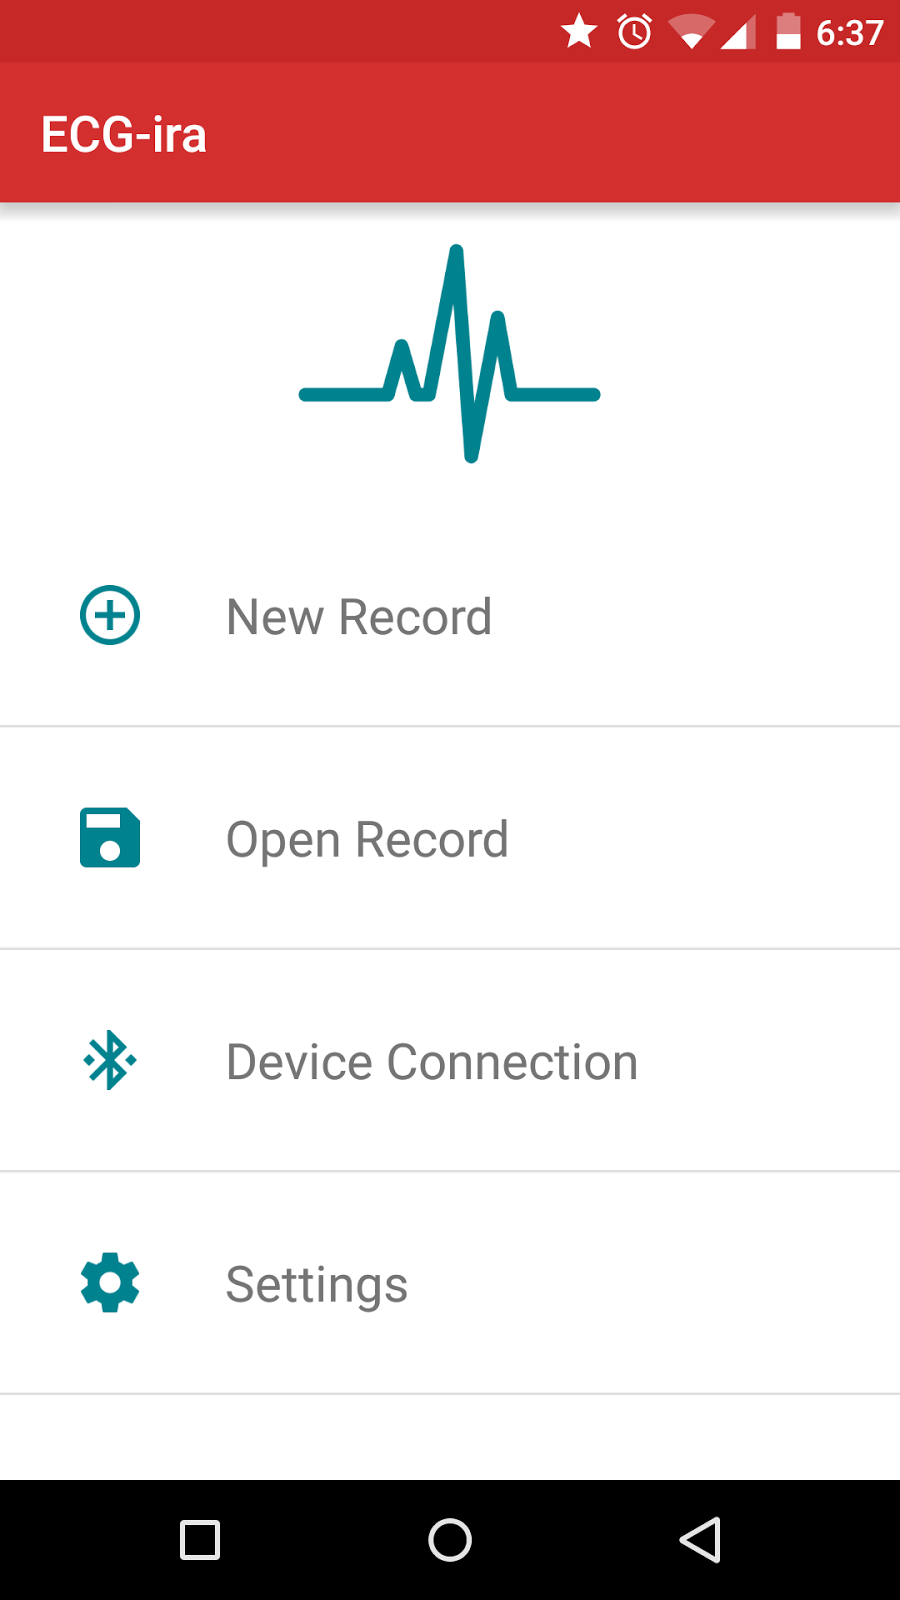
\includegraphics[width=0.3\linewidth]{figures/ch10/1.png}\label{fig10.1}}
\qquad
\subfloat[The form to be compiled before a record can start. It is necessary to bind any record to a patient data in order to avoid confusion between ecg records. This data is also useful for a fully understanding of the record itself]{	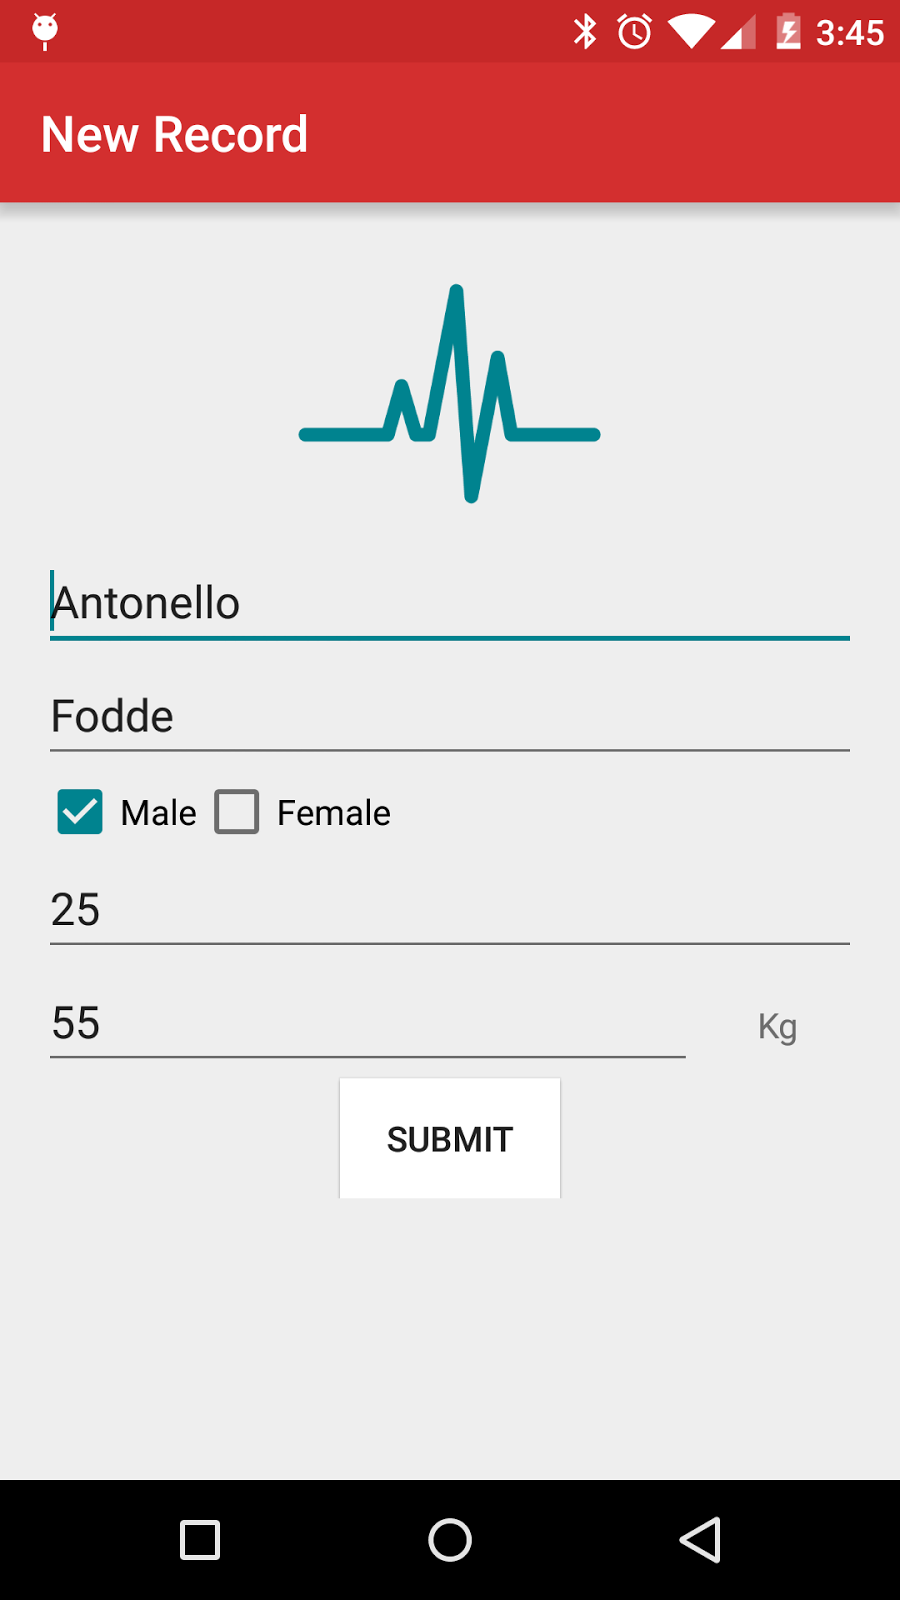
\includegraphics[width=0.3\linewidth]{figures/ch10/2.png}\label{fig10.2}}
\caption{Two screens of the application, respectively the home screen and the form screen to be compiled by the patient}  
\label{fig10.1ab}
\end{figure}
\\By clicking on the “New Record” button option (see figure \ref{fig10.1}), the user will be asked to fill a form with his data as a patient. This data will be then stored within a header file (with .hea extension)  together with the file containing the effective record (.dat file extension). The personal data are only used by the doctor to identify the patient records.
\newpage
Over the submission of the form the file .hea is immediately created to store all the information.\\
If the device is already connected with an acquisition device Zecg, then the application tries immediately to establish a connection to receive data. Otherwise it opens a connection request activity to enable the Bluetooth and start to discover nearby Bluetooth devices.
\newpage
\begin{figure}[!htb]
	\centering
	\subfloat[A real time ECG acquisition from the Zecg acquisition device.]{	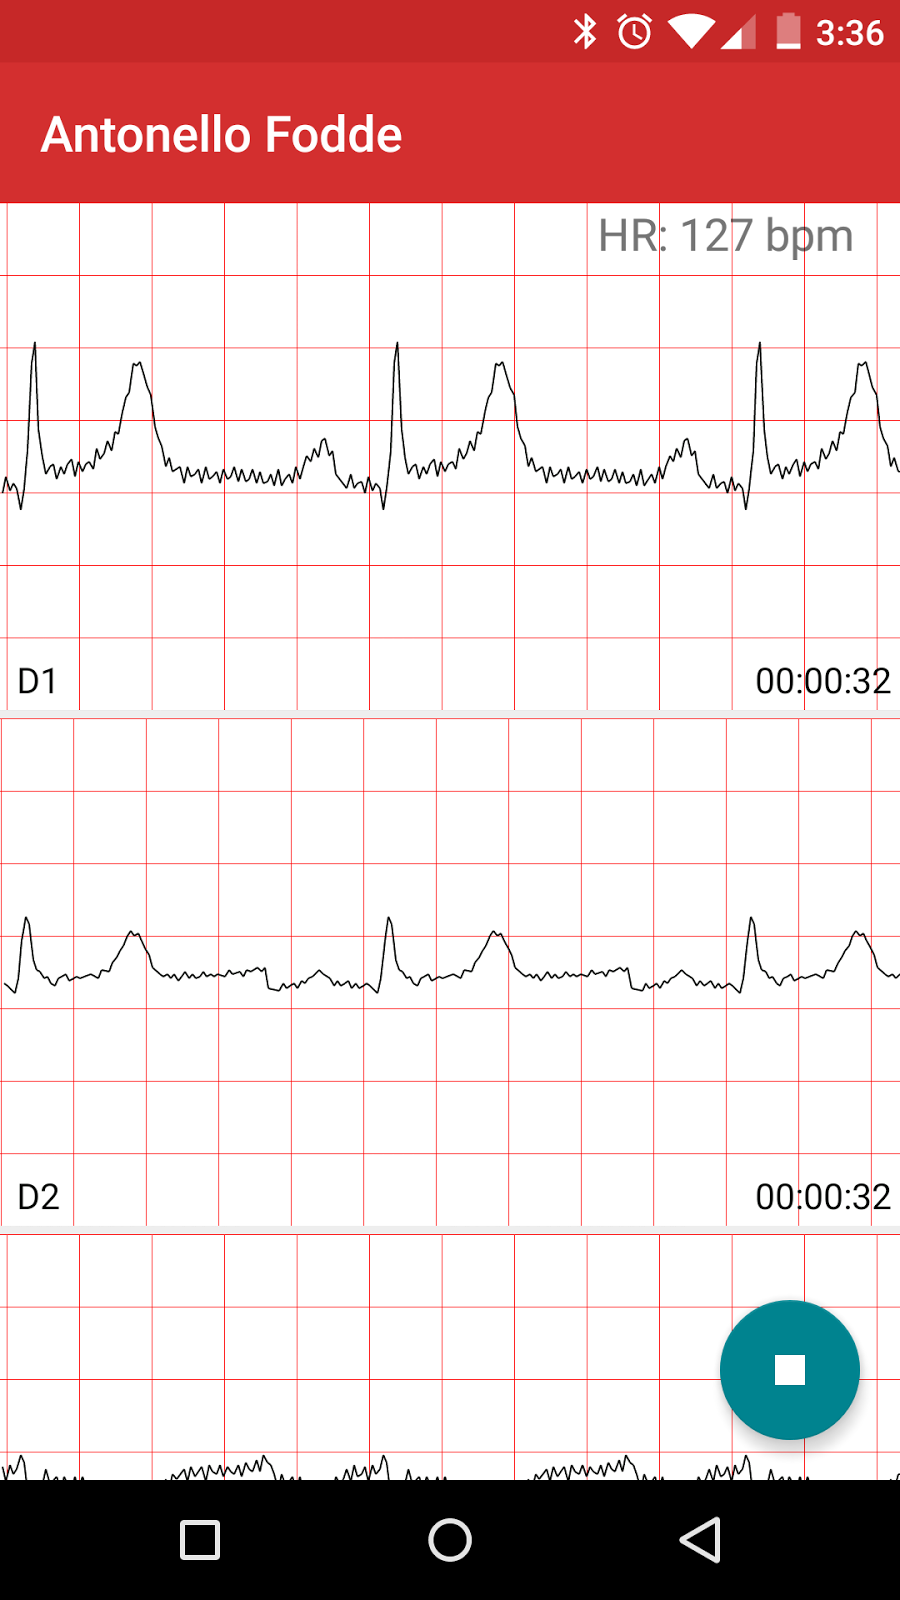
\includegraphics[width=0.3\linewidth]{figures/ch10/3.png}\label{fig10.3}}
	\qquad
	\subfloat[List of records within the device default  folder]{	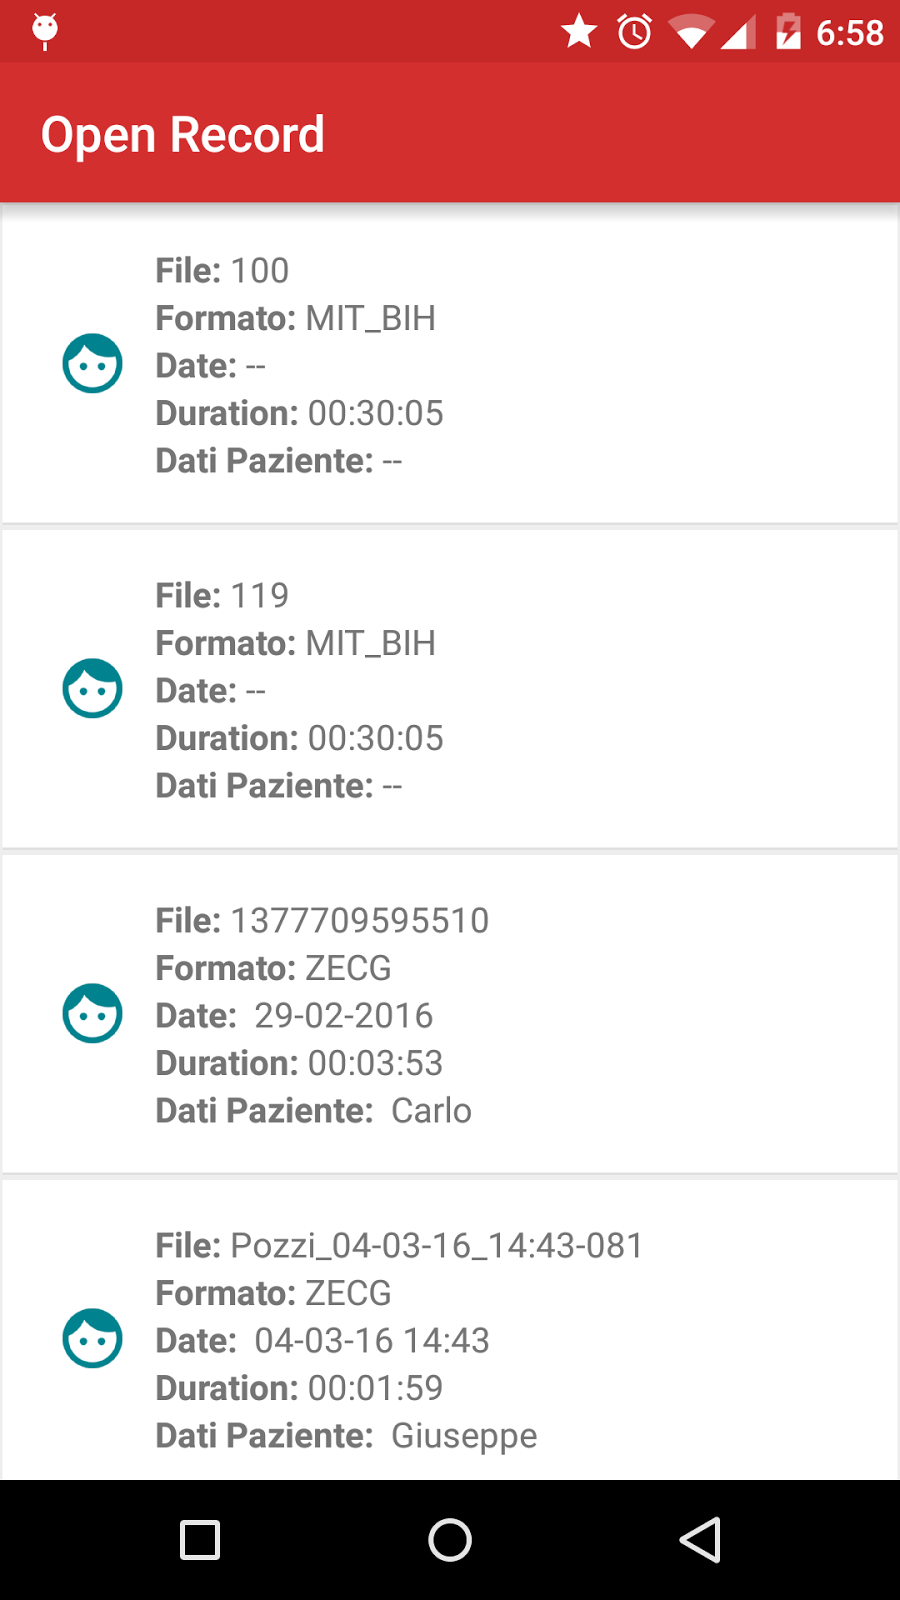
\includegraphics[width=0.3\linewidth]{figures/ch10/4.png}\label{fig10.4}}
	\caption{Two screens of the application representing the realtime acquisition and the list of records within the device}  
	\label{fig10.3ab}
\end{figure}
Going back to the home screen (figure \ref{fig10.1}), by clicking on the “Open record” option button the user will access a list of ECG records saved on its own device on a predefined root folder within the device system memory (the default folder can be changed within the setting section).\\
For each record the most relevant information are highlighted:
\begin{itemize}
	\item File Name
	\item File Format
	\item Acquisition Date
	\item Duration in time of the record
	\item Name of the patient
\end{itemize}	
For more details about each record it is possible to long press on the desired record to show up a ToolBar shown in figure 10.5.
\newpage
\begin{figure}[!htb]
	\centering
	\subfloat[Screen triggered by long pressing on a list item. At the bottom of the screen there is a ToolBar showing the info and the delete options described above.]{	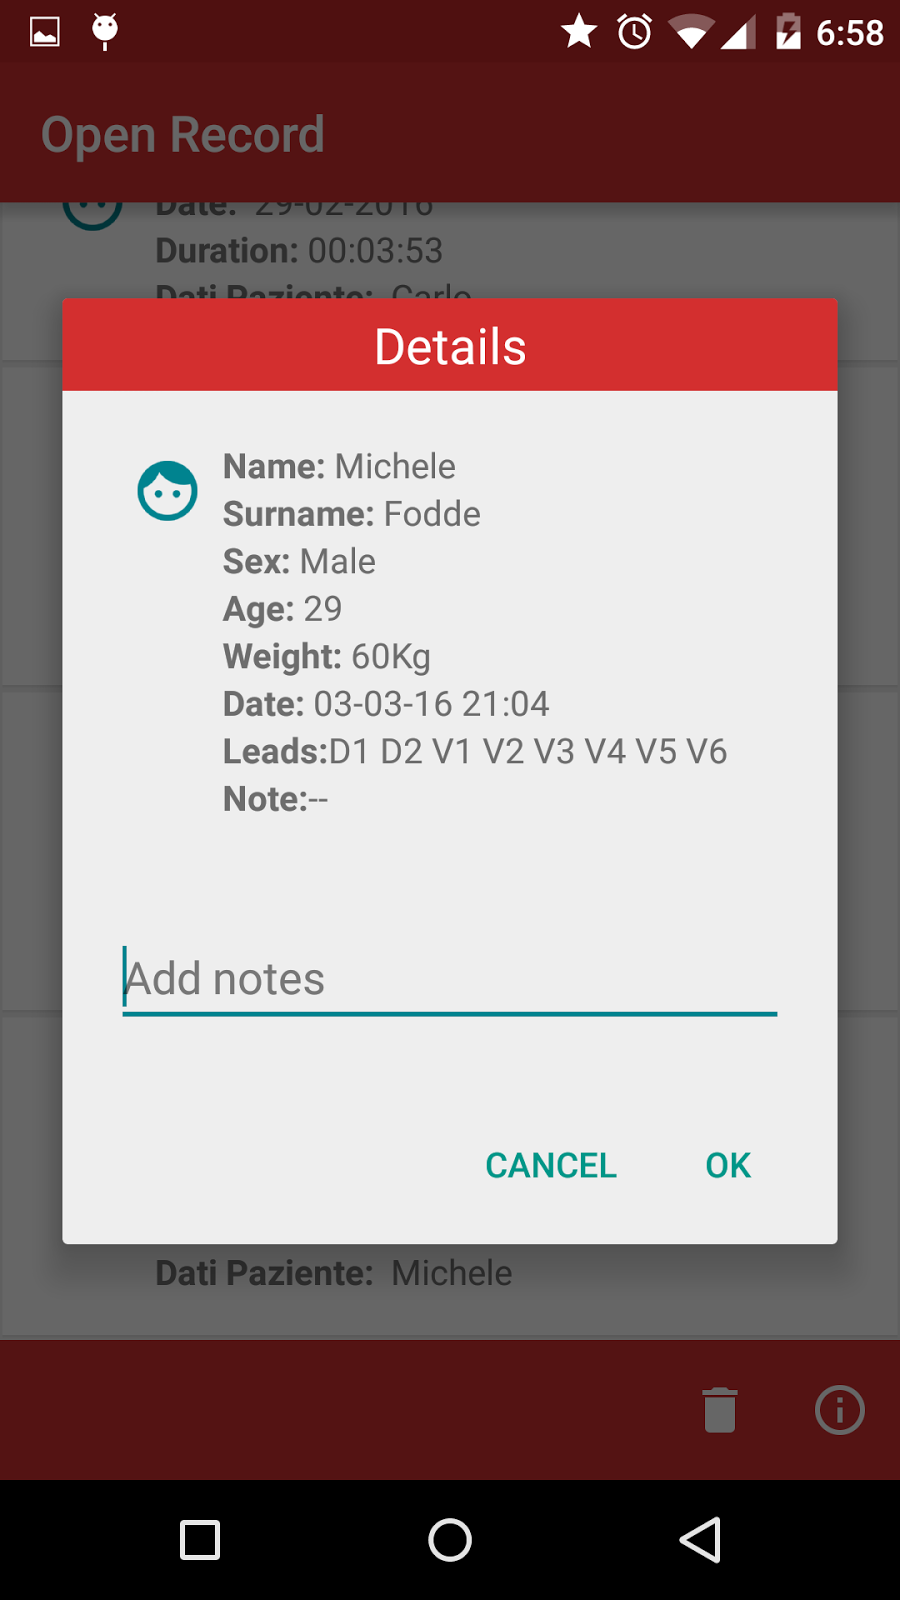
\includegraphics[width=0.3\linewidth]{figures/ch10/5.png}\label{fig10.5}}
	\qquad 
	\subfloat[An example of record opening and plotting. In the screen a MIT-BIH record format was opened.]{	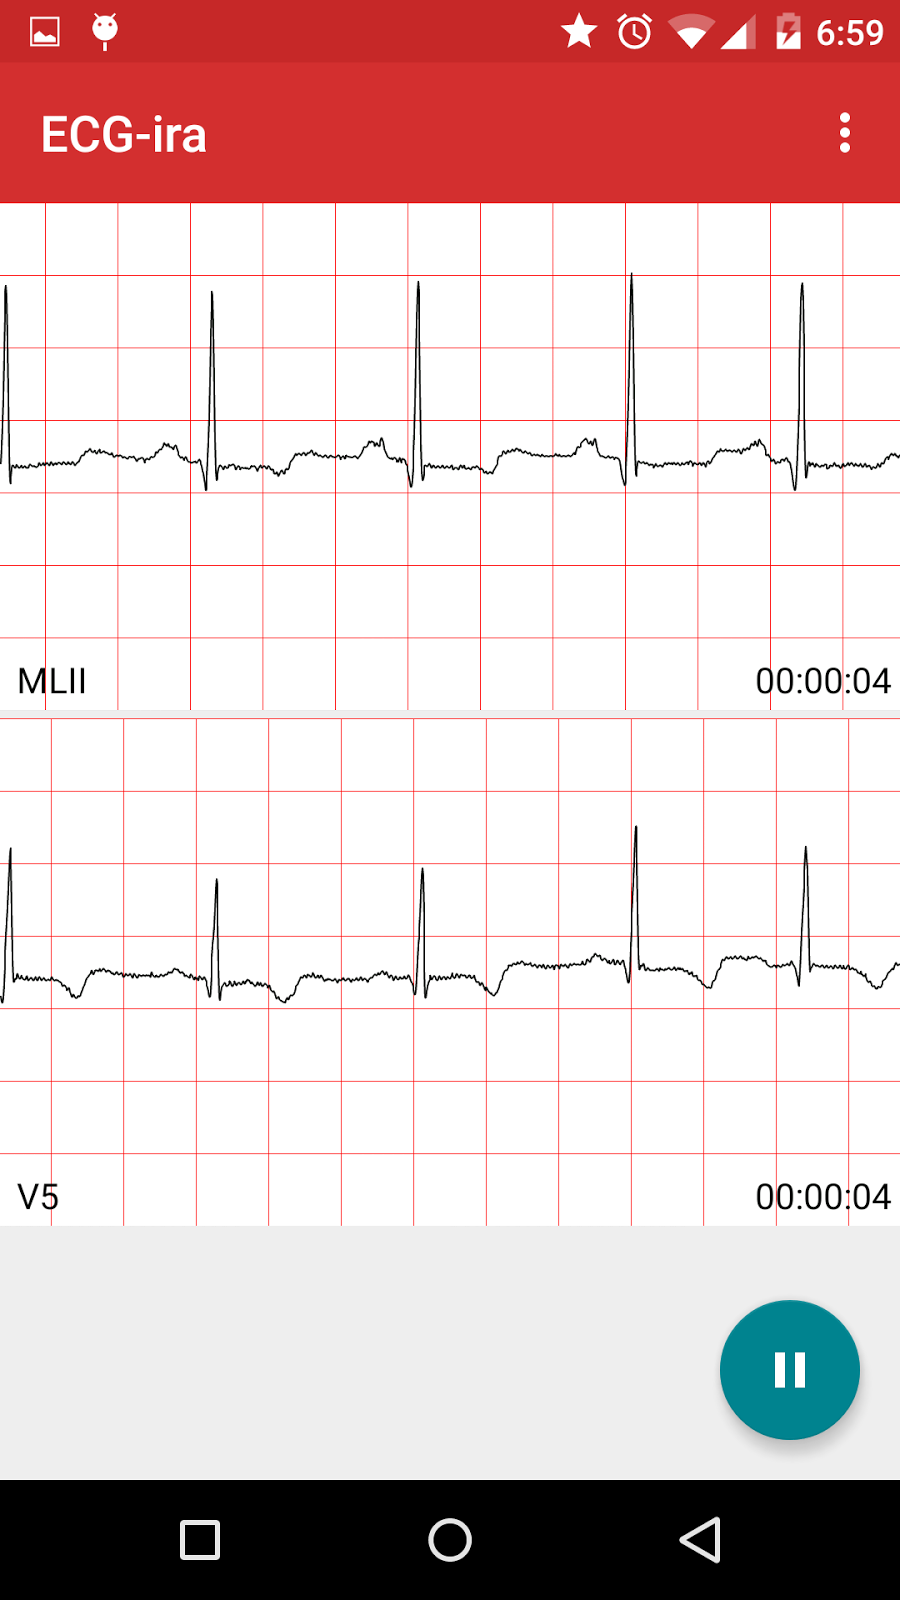
\includegraphics[width=0.3\linewidth]{figures/ch10/6.png}\label{fig10.6}}
	\caption{Two screens of the application representing the info dialog for a certain record and the visualization of that record}  
	\label{fig10.5ab}
\end{figure}
The ToolBar is show at the bottom, it gives the possibility to show more details about the record and the patient information. In the side screenshot the user clicked on the “i” info button so the .hea file containing the user information are shown. Plus the user (in this case the doctor) can add personal notes to the specific record and the specific patient. The notes will be permanently stored within the .hea file.\\
The other option within the ToolBar is a delete record option in case the user decide to remove that specific record, assuming it was taken with too noises or it was just a test record.\\
By opening a record the application will fetch the .dat file and will plot its content over the ECG paper view. It is possible to scroll the record strip just by touching and dragging the screen with a finger, otherwise it is possible to reproduce the record as it was recorded with the exact acquisition speed time by clicking on the green round button at the bottom right.
\newpage
\begin{figure}[!htb]
	\centering
	\subfloat[Progress displaying during the analysis process over the record.]{	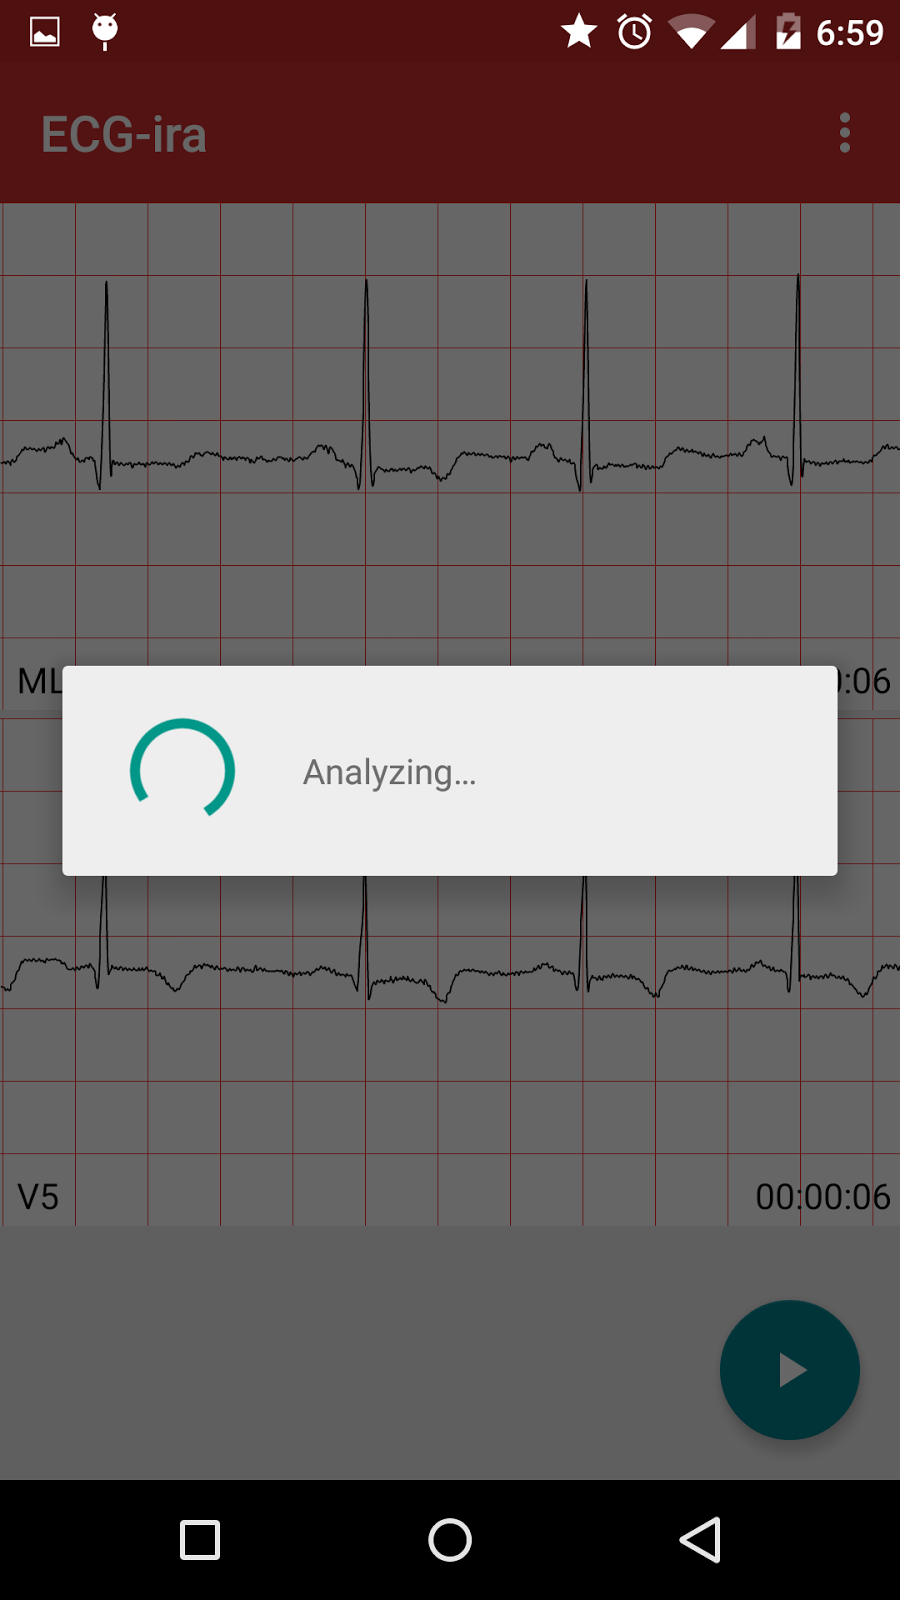
\includegraphics[width=0.3\linewidth]{figures/ch10/7.png}\label{fig10.7}}
	\qquad 
	\subfloat[Screen of the record plot with annotations results from an analysis over the first lead (MLII).]{	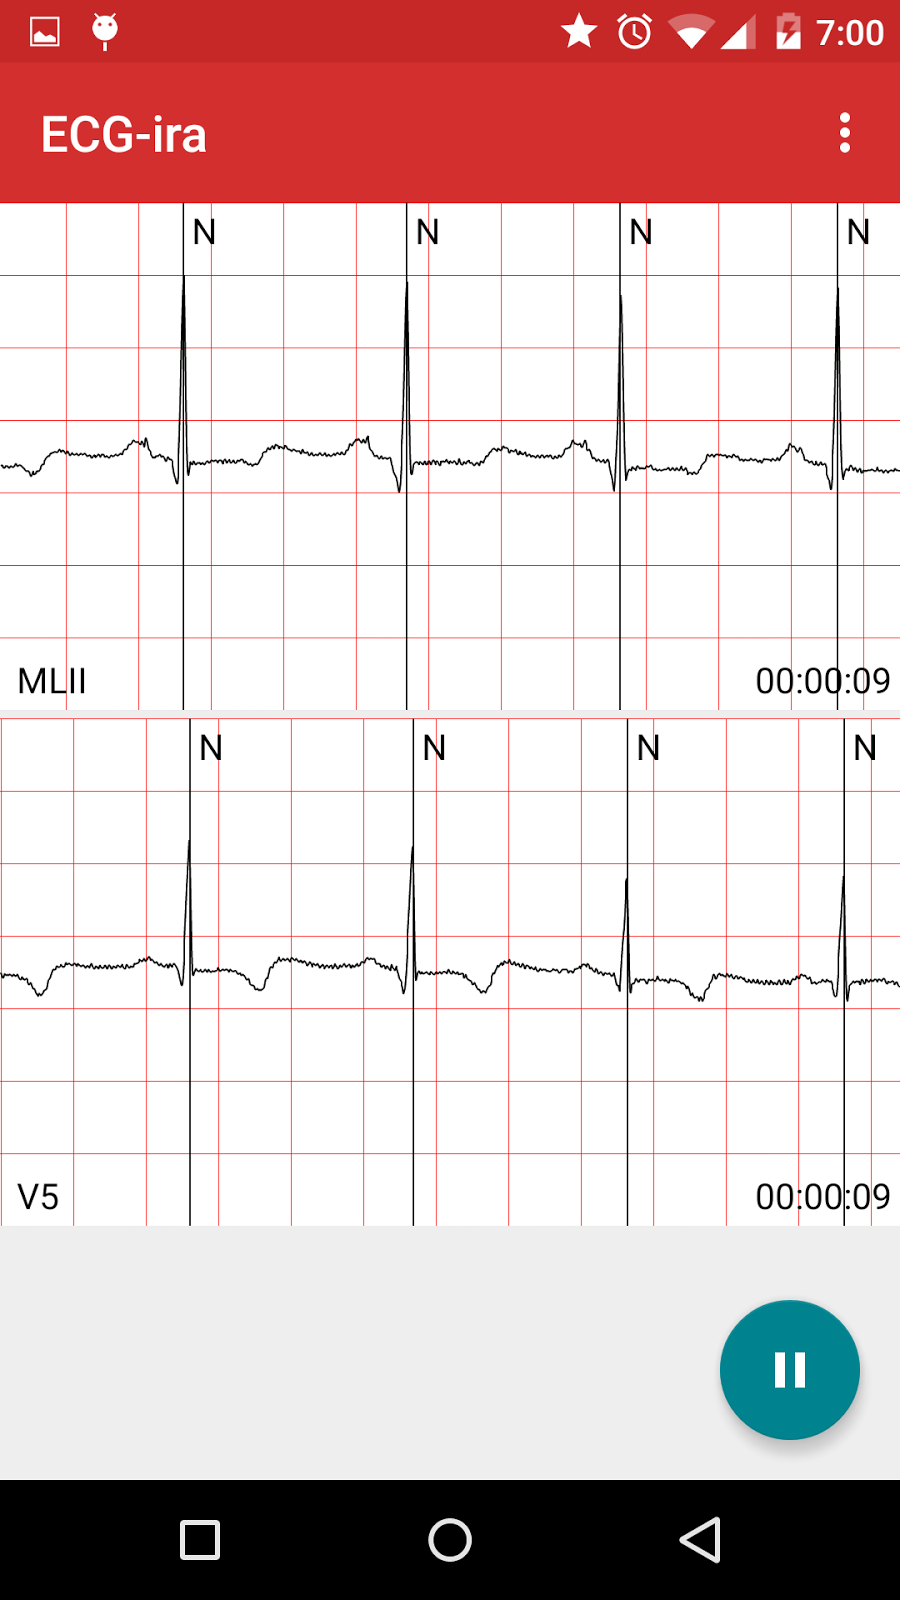
\includegraphics[width=0.3\linewidth]{figures/ch10/8.png}\label{fig10.8}}
	\caption{Two screens of the application representing the info dialog for a certain record and the visualization of that record}  
	\label{fig10.7ab}
\end{figure}
The top ToolBar option menu is used to trigger the analysis algorithm over the opened record. If the user triggers this command, due to the great amount of operations behind the analysis process we force the user to wait for the result till the process ends. \\
The result of an analysis is the plot of the annotation letters (N=normal, V=ventricular, A=atrial) related to each detected beats and its diagnosis.  In the screenshot we can see four heart beats marked as Normal. The annotations covers all the record length and even if it is done on one lead only (D2 as default analysis signal), it is shown on all the other leads.
\newpage
\begin{figure}
\centering
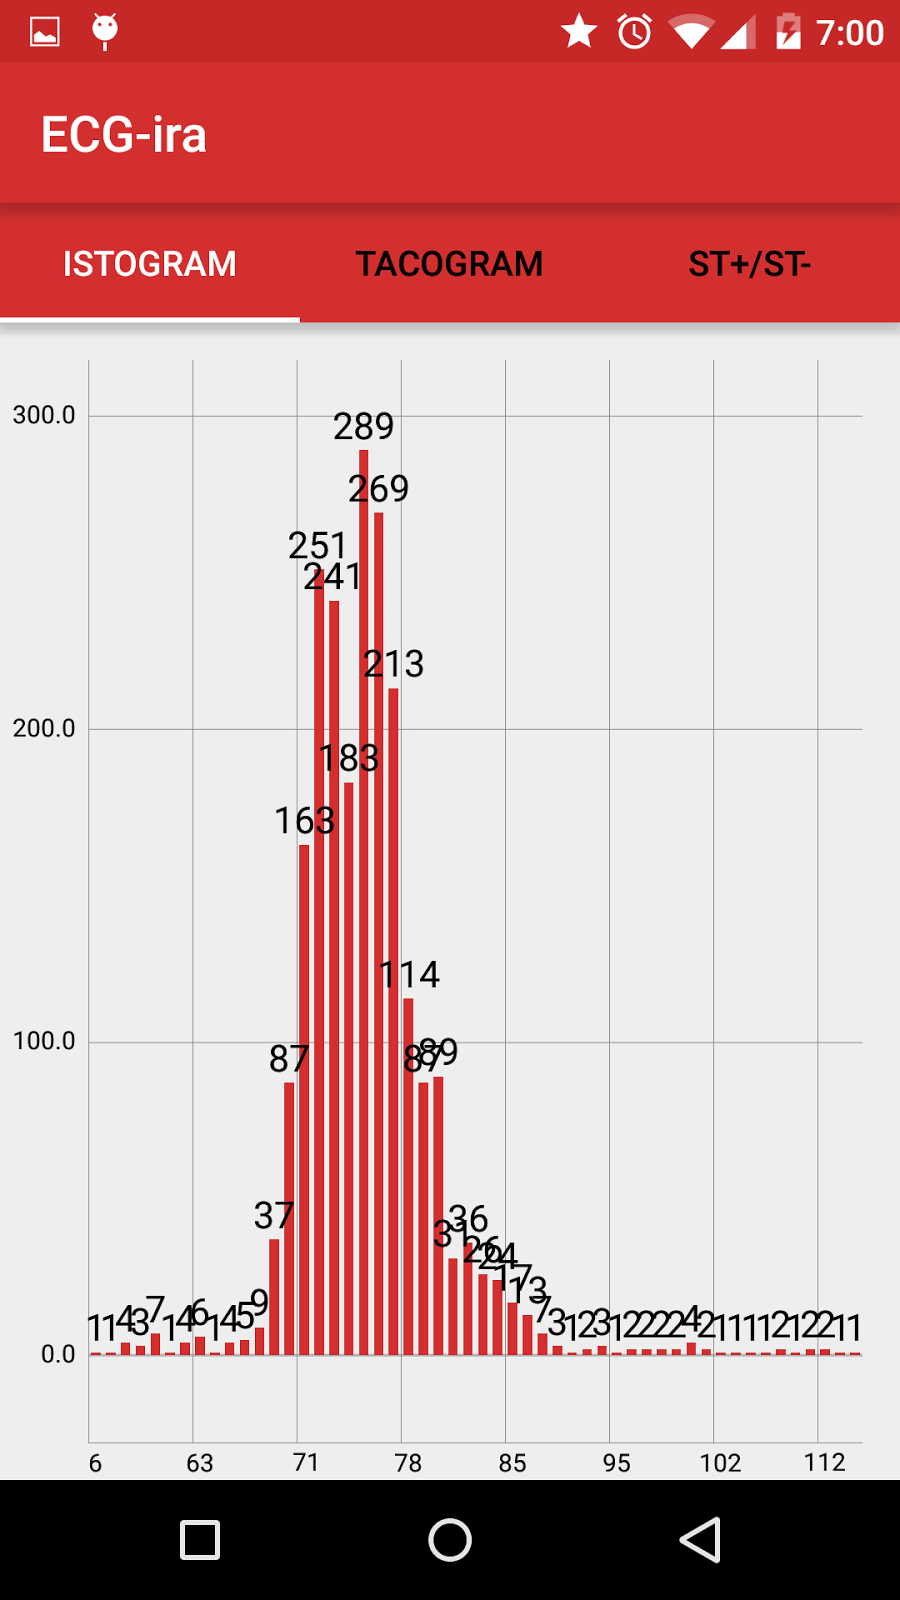
\includegraphics[width=0.3\linewidth]{figures/ch10/9.png}
	\caption{Screen of the three graphs generated after an analysis of the records. They are graphs summing up the complete record characteristics. Useful for a general overview of the patient record and health status.}  
	\label{fig10.9}
\end{figure}
Another result from the analysis is the generation of three different graphs useful to support a better analysis over the heart overall behaviour as they sum up the total record “statistics”. They are:\\
\begin{itemize}
\item \textbf{Istogram} : on the X-axis we have an ordered values of the heart beats measures in bpm. On the Y-axis the occurrences of beats at that bpm value.
\item \textbf{Tacogram}: on the X-axis we have the number of heartbeats retrieved by the analysis. On the Y-axis the bpm values of each heart beats. 
\item \textbf{ST+/ST-}: this graph shows instead, for each heartbeat, the amount of area below the ST segment and the area above that segment. This is useful especially to detect some specific arrhythmias.
\end{itemize}
\newpage
\begin{figure}[!htb]
	\centering
	\subfloat[First parameters option within the Custom Settings]{	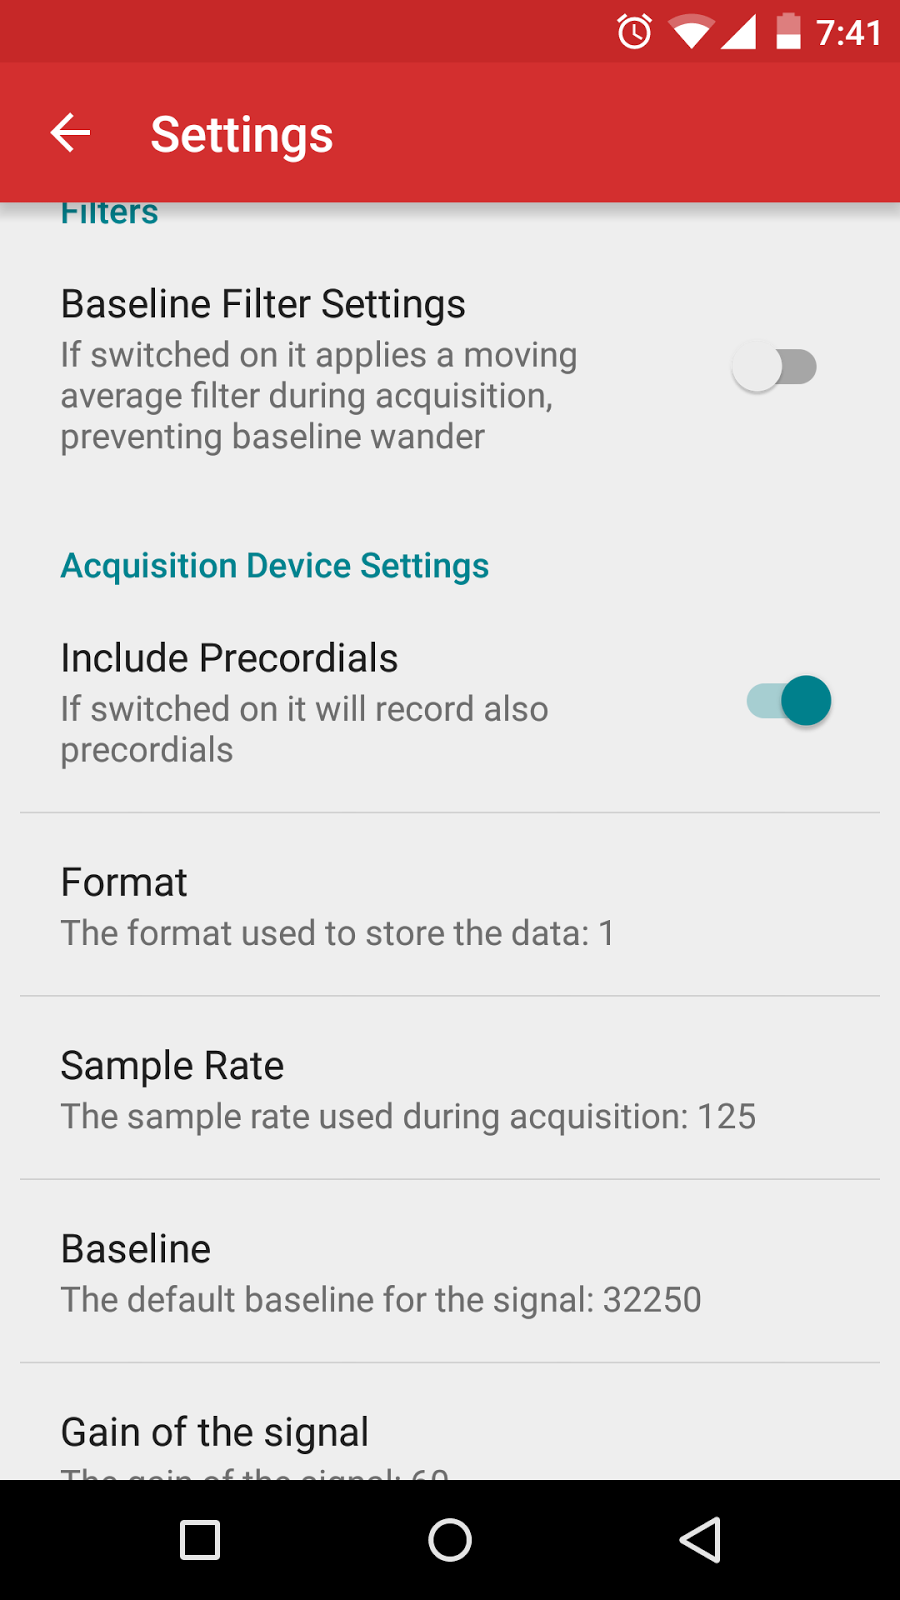
\includegraphics[width=0.3\linewidth]{figures/ch10/10.png}\label{fig10.10a}}
	\qquad 
	\subfloat[Second parameters option within the Custom Settings]{	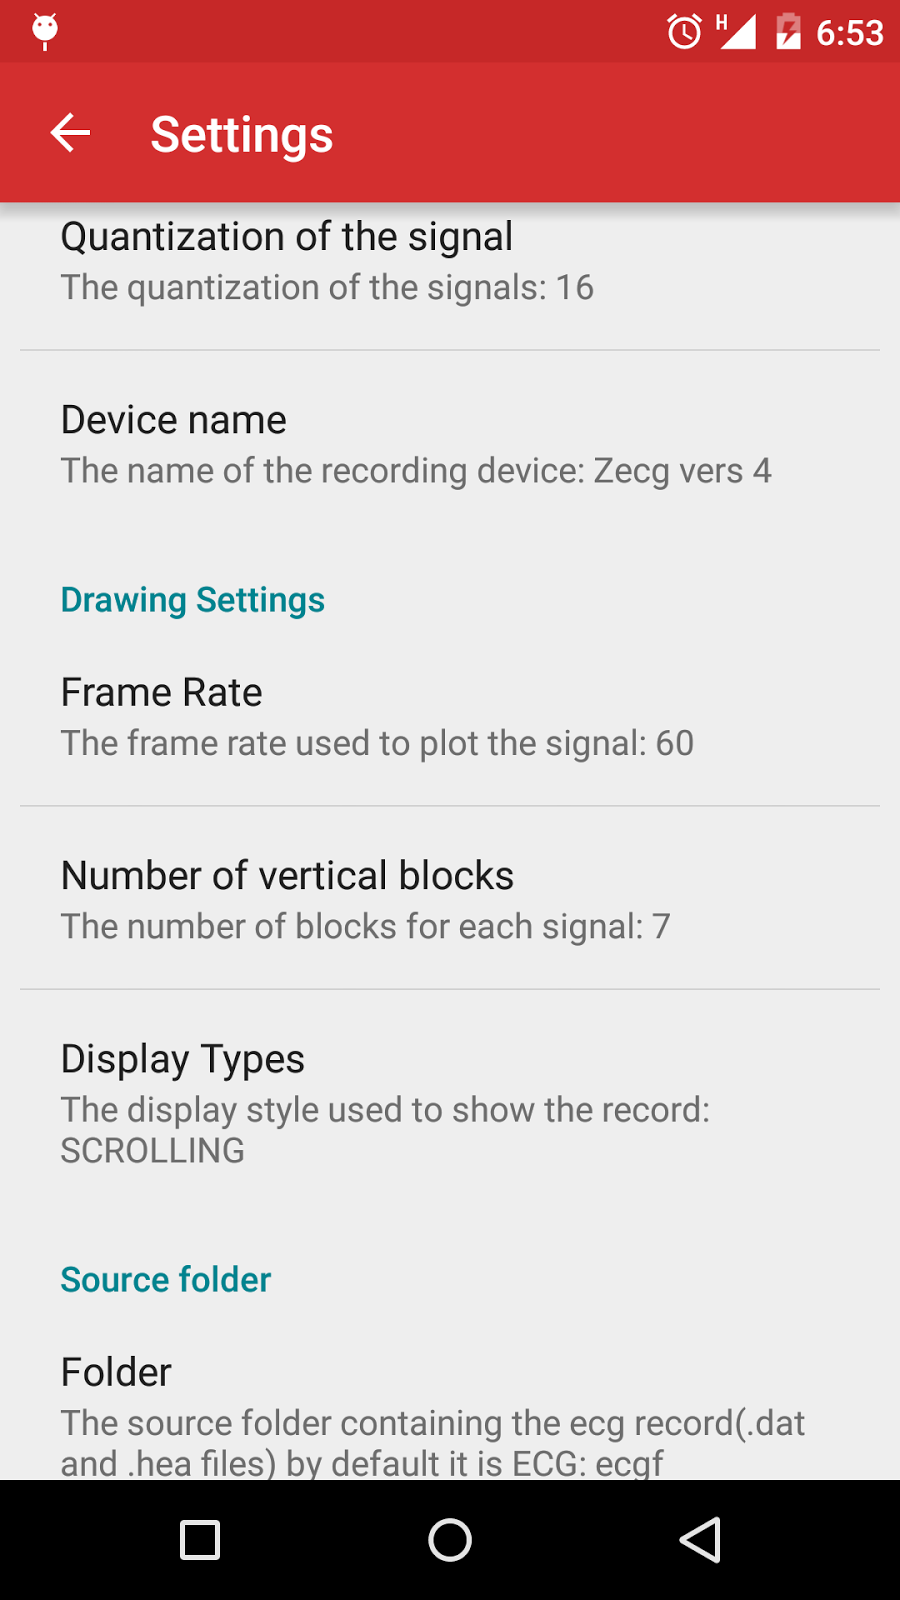
\includegraphics[width=0.3\linewidth]{figures/ch10/10b.png}\label{fig10.10b}}
	\caption{The customization section of the application. A list of available settings parameters to tune the application behaviour.d}  
	\label{fig10.10}
\end{figure}
About the customization setting  for the application we made a long setting screen with lots of customizable parameters.\\
The first is related to the application of a baseline filter during the record visualization in order to reduce the baseline wandering effect. The second category of settings are related to the acquisition phase. It includes the acquisition format, the gain, the sample rate, quantization and the name of the acquisition device (for example it can be: ZEcg vers 2/3/4).\\
The third category is related to the drawing settings. These settings will affect only the graphical views such as the height of each strips, the way the strip is reproduces (by scrolling or by using the old style oscilloscope effect) and the preferred frame rate to be used.\\
The last category is to tune the default folder to store the new acquired records and from which open the records within the application (figure \ref{fig10.4}).
\subsection{Performance}
In this section we reported some performance results from different aspects such as Memory usage, CPU usage and response time during a run of the application performed on different devices with installed different Android OS and different hardwares. The tests were performed on the following devices dated respectibely on 2011 and on 2015:
\begin{itemize}
	\item Samsung Galaxy Note N7000
	\item OnePlus X
\end{itemize}
The table \ref{tab10.1} shows the specification details of these 2 smartphones.\\
\begin{table}[h!]
	\centering
\begin{tabularx}{\textwidth}{|X|X|X|}
	\hline
		\textbf{Model}  & OnePlus X & Samsung Galaxy N7000  \\ \hline
		\textbf{Brand}  & OnePlus & Samsung \\ \hline
		\textbf{Year}  & November 2015 & October 2011 \\ \hline
		\textbf{Display Type}  & AMOLED capacitive touchscreen, 16M colors & Super AMOLED capacitive touchscreen, 16M colors \\ \hline
		\textbf{Display Size}  & 5.0 inches & 5.3 inches \\ \hline
		\textbf{Resolution}  & 1080 x 1920 pixels (~441 ppi pixel density) &  800 x 1280 pixels (~285 ppi pixel density) \\ \hline
		\textbf{OS}  & Android OS, v5.1.1 (Lollipop) & Android OS, v4.1.2 (Jelly Bean) (upgraded from v2.3.5) \\ \hline
		\textbf{CPU}  & Quad-core 2.3 GHz & Dual-core 1.4 GHz Cortex-A9 \\ \hline
		\textbf{Memory(internal)}\vline  & 16 GB & 16 GB \\ \hline
		\textbf{RAM}  & 3 GB & 1 GB \\ \hline
		
	\end{tabularx}
	\caption{The two test devices specification details.}
	\label{tab10.1}
\end{table}
The results are not to be considered absolutely valid for all the above device families. The performance can be affected by many different factors that may not be related with the applications itself; hence the results may vary from a test to another. Since Android OS is in charge to manage the system memory and split the available resources between all the installed applications, having our application on foreground doesn’t necessary mean we can reserve all the power and memory resource for our business. Part of the system resources are allocated to run the Garbage Collector which itself has its own timing when cleaning and deallocating other application resources. Then all the applications having background tasks also need to be kept alive, for example notification services or messaging services.\\
It is not easy to measure the application performance in a clean absolute way, harder is to compare the results coming from different devices, that is why we will only report the results related to each devices and we will analyze how the application performs on each.
\subsection{Evaluation}
We evaluated the performance considering three application states:
\begin{itemize}
	\item \textbf{Idle state}: the application is open on a simple basic screen such as the home screen or the record list screen.
	\item \textbf{Plotting state}: the application is performing a plotting of a record
	\item \textbf{Analysis state}: the analysis algorithm is performed over the record
\end{itemize}
\subsubsection{Memory}
Before going in details about the memory usage result for the application performing on the different devices, there is some basics knowledge about the analysis tools used and the way to read them that the reader should be aware of.\\
Android Studio provides a Memory Monitor Tool allowing the user to track how his application performs in term of memory usage. Apart of a generic view of memory usage there is a more detailed view that let you observe how your app’s memory is divided between different types of RAM allocation.
The most important and relevant values to care of are: 
\begin{itemize}
	\item Private (Clean and Dirty) RAM: The memory being used by ONLY your process. This is the bulk of the RAM that the system can reclaim when your app’s process is destroyed. The most important is the private dirty RAM, which is the most expensive because it is used by only your process and its content exists only in RAM so it can’t be paged to storage. (Android does not use SWAP). All Dalvik and native heap allocations you make will be private dirty RAM; Dalvik and native allocations you share with the Zygote process are shared dirty RAM.
	\item Proportional Set Size (PSS): This is a measurement of your app’s RAM use that takes into account sharing pages across processes. Any RAM pages that are unique to your process directly contribute to its PSS value, while pages that are shared with other processes contribute to the PSS value only in proportion to the amount of sharing. For example, a page that is shared between two processes will contribute half of its size to the PSS of each process.
	\item Dalvik Heap: The RAM used by Dalvik allocations in your application.
	\item .so mmap and .dex mmap: The RAM used for mapped .so (native) and .dex (Dalvik or ART) code.
	\item .art mmap: Amount of RAM used by the heap image which is based off the preloaded classes which are commonly used by multiple apps. It does not count towards your app heap size.
	\item .Heap: The amount of heap memory for your application.
\end{itemize}
\begin{figure}[h!]
	\centering
	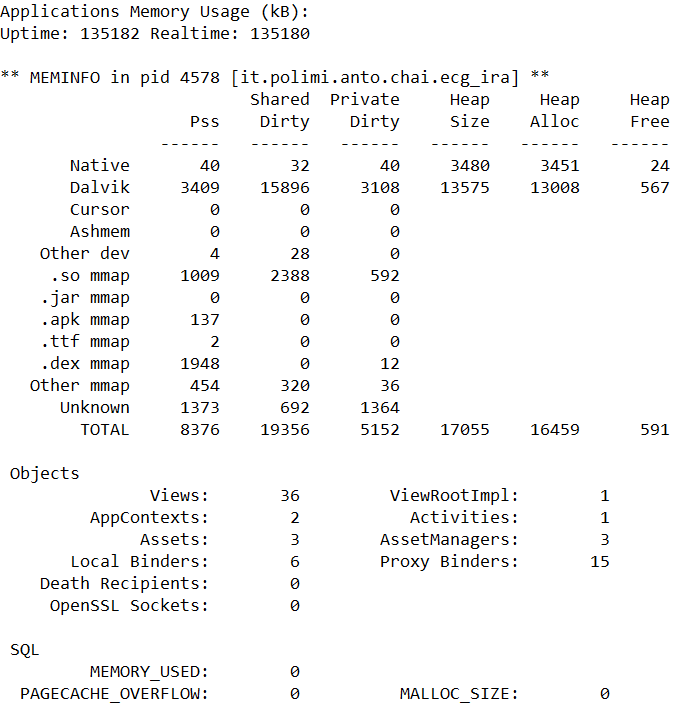
\includegraphics[width=0.6\linewidth]{figures/ch10/12.png}
	\caption{An example of detailed view of an application memory usage.}  
	\label{fig10.12}
\end{figure}
The memory tests were executed running the application on the same screens and opening and plotting always the same record. It was used the 100.dat from MIT/BIH format because it is the longest and biggest record.
\paragraph{Samsung Galaxy N7000}
This is the oldest device according to its release date. To make this device compatible with the minimum API requirement (API 16)  the device was upgraded to android Jelly Bean (API 16).\\
The hardware instead was the same from the manufacturer since its release on 2011. \\
During the test the device performed quite well. It never crashed due to memory leakage or Out of Memory Exception.\\
Let’s start observing the memory usage during the three application states:
\subparagraph{Idle state}
The memory usage looked constant over the time as expected.
\begin{figure}[h!]
	\centering
	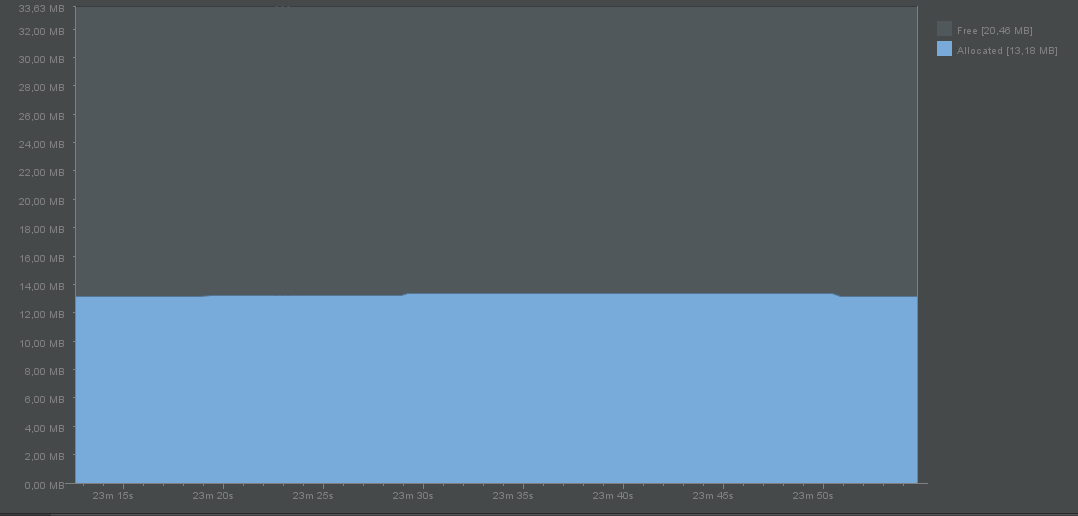
\includegraphics[width=1\linewidth]{figures/ch10/13.png}
	\caption{Memory usage during application idle state. It is quite constant (due to user interaction it can slightly increase or decrease if no interaction at all for a while).}  
	\label{fig10.13}
\end{figure}
The memory usage graph above shows the actual memory stack allocated for the application and how many of that is used by the application.  As it can be seen on the top right the application is using 13.18 MB and 20.46 are still free. The total device  memory is not shown. In case the application hits the upper bound, let’s say it occupies the other  free 20.46 MB, then the OS will allocate more memory for the actual application by garbage collecting resources from other background applications or actually killing other low priority processes (all the processes not in foreground are considered with lower priority).
\newpage
Here are more detailed information about the memory usage and resources allocations during idle state:
\begin{figure}[ht]
	\centering	
	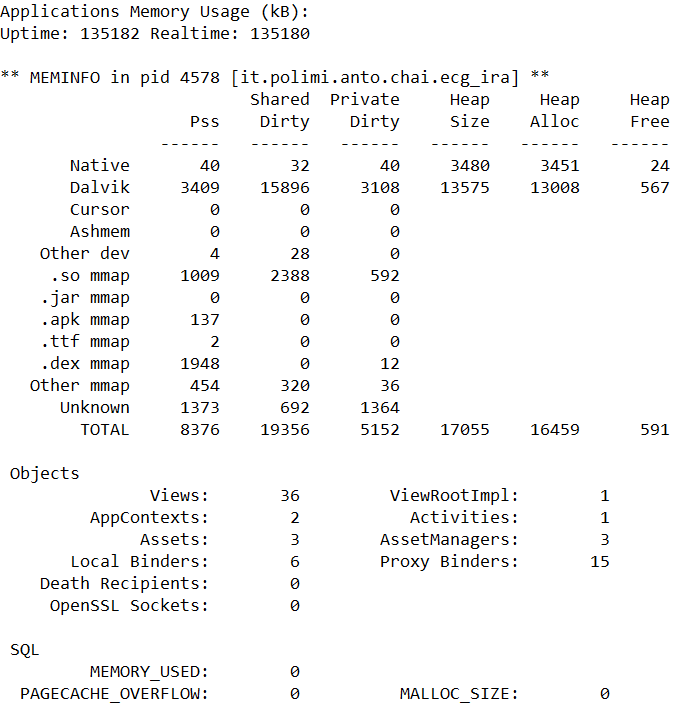
\includegraphics[width=0.6\linewidth]{figures/ch10/14.png}
	\caption{Details about memory usage and allocation over the different RAM section for the application EC-ira.}  
	\label{fig10.14}
\end{figure}
\subparagraph{Plotting state}
During a record plotting the memory usage increases since the drawing process itself consume memory by allocating new resources and by the resource manipulations and usage.\\
The waves in the memory usage graph (figure \ref{fig10.15} are due to the garbage collector calls which free unused resources. This is really an interesting  Garbage Collecting behaviour, because we can observe it collecting resources with a certain regularity rate (somehow very often).\\
The detailed information about memory usage divided by types of RAM used are shown in the figure \ref{fig10.16}.
\begin{figure}[!htb]
	\centering
	\subfloat[Memory usage during a record plotting. The waves are due to Garbage collector calls to free resources. The final resource usage in this phase is rather constant as well.]{	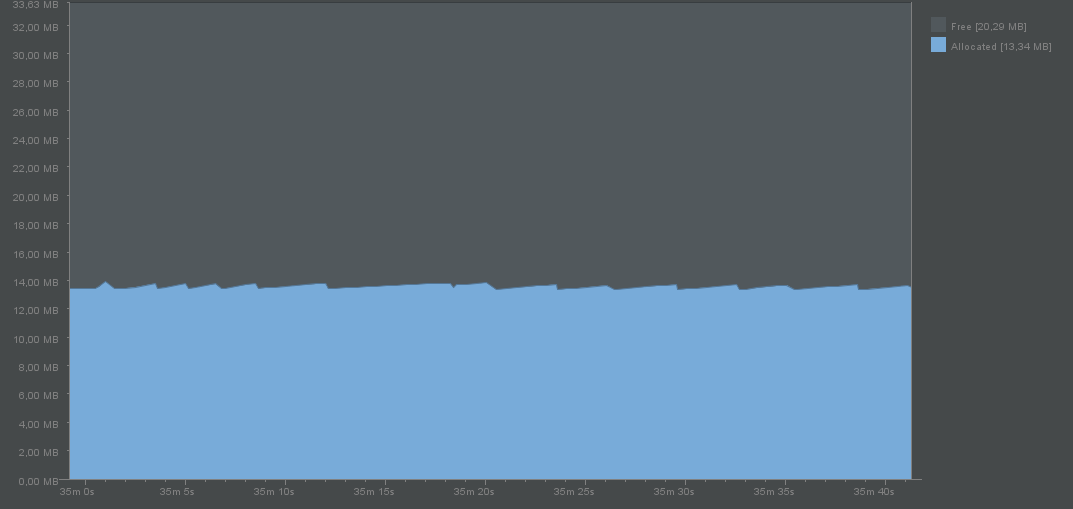
\includegraphics[width=1\linewidth]{figures/ch10/15.png}\label{fig10.15}}
	\\
	\subfloat[Memory usage by RAM types during a record plot.]{	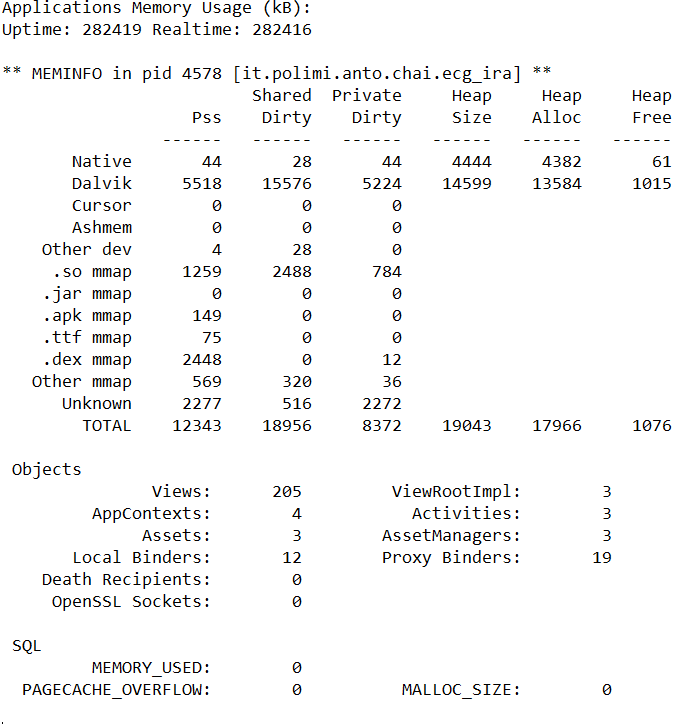
\includegraphics[width=0.6\linewidth]{figures/ch10/16.png}\label{fig10.16}}
	\caption{Two memory usage views, relatively the realtime view with the application running and the per process memory view and allocation.}  
	\label{fig10.15ab}
\end{figure}

The Private Dirty Dalvik in increased from Idle state from 3108 kB to  5224 kB. The TOTAL Pss increased from 8376 kB in Idle state to 12343 kB during  a plot.
\newpage
\subparagraph{Analysis state}
This is the most interesting part of the memory usage results. We can clearly distinguish the application behaviour just by looking at the memory stack. The analysis is the more complex and intensive memory usage step.
\begin{figure}[h]
	\centering	
	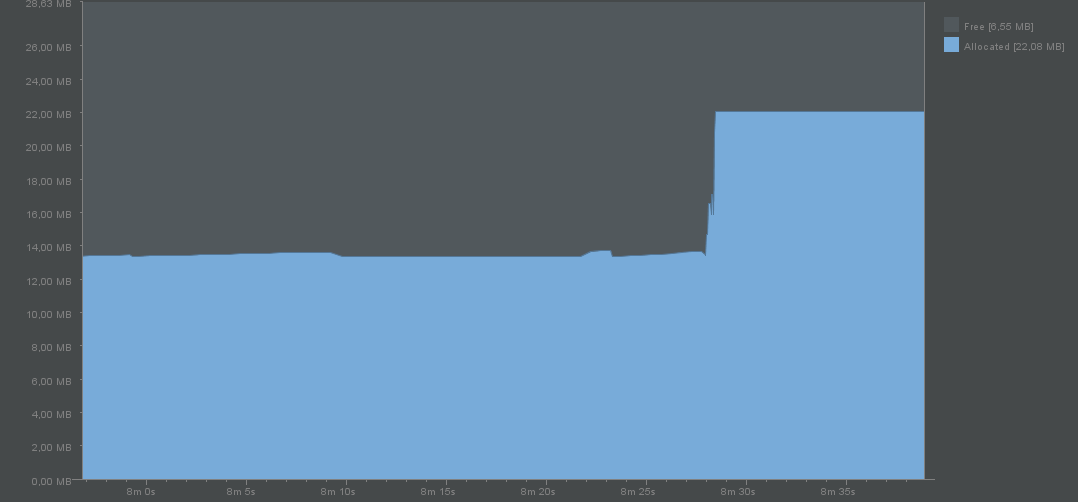
\includegraphics[width=1\linewidth]{figures/ch10/17.png}
	\caption{Memory usage during an analysis launched over a record. The step is due to the record allocation in a memory buffer.}  
	\label{fig10.17}
\end{figure}
\newline At seconds 0m 28s  the user clicked on the analysis button. The peak on the memory usage graph is due to the creation of the buffer to store the entire record in order to perform the analysis algorithm on it. 
\begin{figure}[h!]
	\centering	
	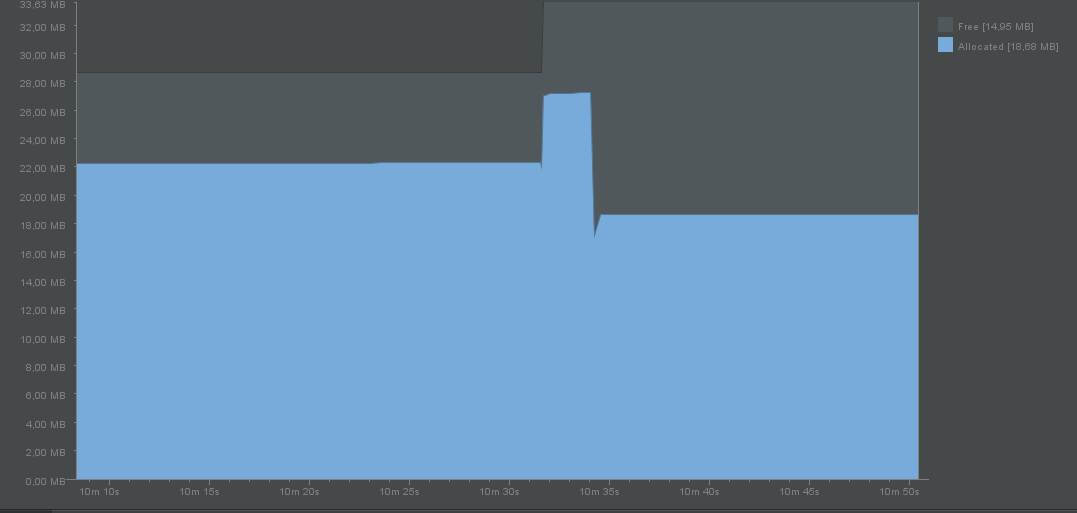
\includegraphics[width=1\linewidth]{figures/ch10/18.png}
	\caption{ Memory usage at the exact time the algorithm performs the final steps by computing the ST+/St- areas (execution finish at 10m34s).}  
	\label{fig10.18}
\end{figure}
At 10m34s the analysis algorithms finish to perform. More resources are instantiated for computational purpose of the algorithms. As at 10m34s the algorithms terminate, all the resources can be freed and only results are returned.\\
As you can see in the memory usage graph, the OS kind of predicted or expected the application to require and allocate more resources, so it allocates more spaces for it even if the upper bound of 28.40 MB wasn’t reached. But as soon as the resources allocated were of no use anymore, it triggered the Garbage Collector to free them.\\
In figure \ref{fig10.19} is the detailed information about the overall memory usage which is divided by RAM types.
\begin{figure}[h]
	\centering	
	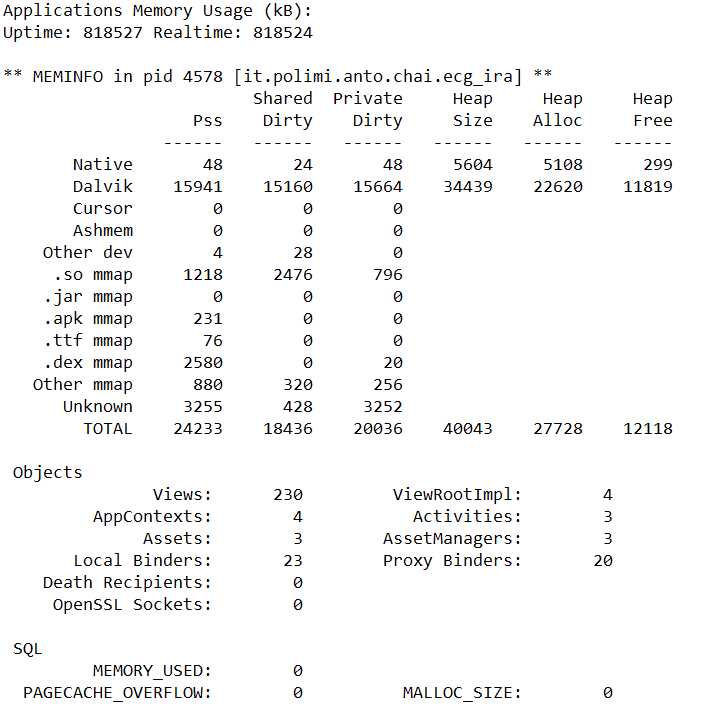
\includegraphics[width=0.6\linewidth]{figures/ch10/19.png}
	\caption{ Memory usage details by RAM types.}  
	\label{fig10.19}
\end{figure}
We can easily observe that the Private Dirty Dalvik became the triple with respect to its size during the plotting phase (5224 kB --> 15664 kB) and the TOTAL Pss doubled. This behaviour is due to the record copy into memory and all the data structures used to compute the analysis.\\
Much of the other field didn’t changed their values nor allocation size, for example the .so mmap was the same both in the plotting state both in the analysis state.\\
\\
As final result we can conclude that during the entire process and states of the application ECG-ira on the Samsung Galaxy N7000, the application performed fairly well consuming resources as it needed and releasing them as soon as possible. We observed also that the OS Garbage Collector overall behaviour was to trigger as often as possible as soon as the resources in no more used.
\paragraph{OnePlus X}
This device  is the most advanced one we tested the application on. With it’s 3GB RAM memory and its powerful quad-core processor we really  expect no issues, but let’s dig into the results.\\
For a better understand of some terms, you are invited to read the introduction of the Memory Chapter.
\subparagraph{Idle state}
The idle state is as well predictable,  the memory usage is stable.
\begin{figure}[h!]
	\centering	
	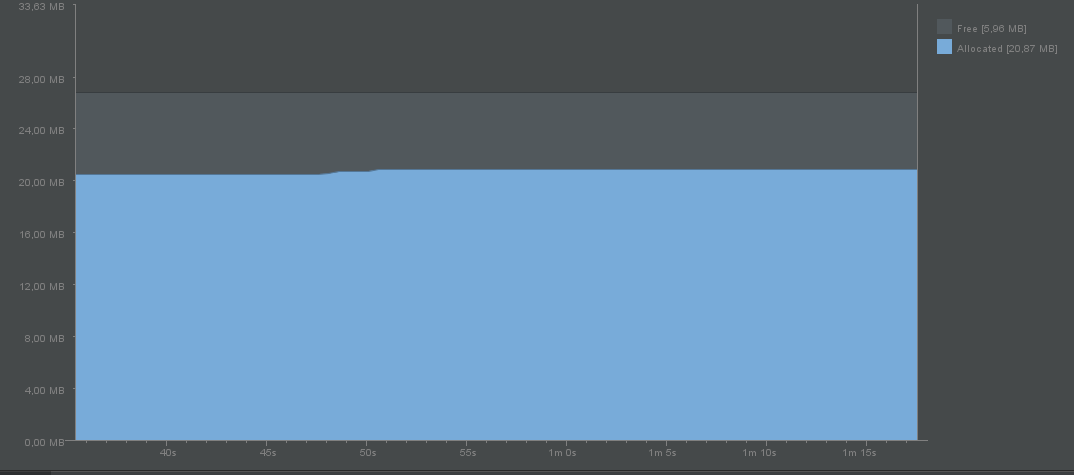
\includegraphics[width=1\linewidth]{figures/ch10/20.png}
	\caption{ Memory usage of ECG-ira in Idle state.}  
	\label{fig10.20}
\end{figure}
It is relevant to observe that the device consume much more memory (20.87 MB) with respect to the idle state values measured on the Samsung Galaxy N7000 (13.18 MB). This can be explained with the fact that firstly the two OS are firstly completely different and rely on different API. The OnePlus X device relies on the API 21 while the Samsung N7000 on API 16. Also the screen size and pixels density is not comparable since the OnePlus X doubles the old Samsung device.\\
Apart using more resources the final result is the same since the idle state doesn’t show any memory leakage. More information are provided in the figure \ref{fig10.21}.
\begin{figure}[h!]
	\centering	
	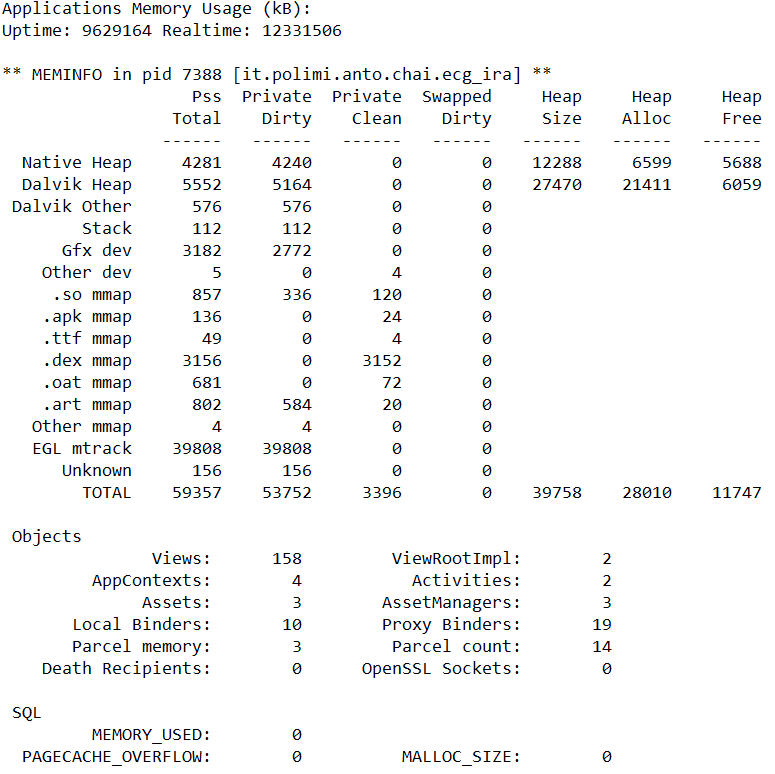
\includegraphics[width=0.6\linewidth]{figures/ch10/21.png}
	\caption{ Memory usage of ECG-ira in Idle state by RAM types.}  
	\label{fig10.21}
\end{figure}
An interesting data from the above table is that the Private Dirty Native Heap and the Private Dirty Dalvik Heap are really close to have the same value. This means that some views used inside the application makes use of the Graphical layer offered by OpenGL (it means they are hardware accelerated). Actually most of the Total Pss and Private Dirty allocations comes from the EGL mtrack, in other words it refers to the memory consumed by Graphics layer.
\subparagraph{Plotting state}
During the plotting phase we can observe a different Garbage Collector behaviour with respect to the one observed on the Samsung N7000.
\begin{figure}[!htb]
	\centering
	\subfloat[Memory usage during a record plotting. We can see that the step is due to a GC call.]{	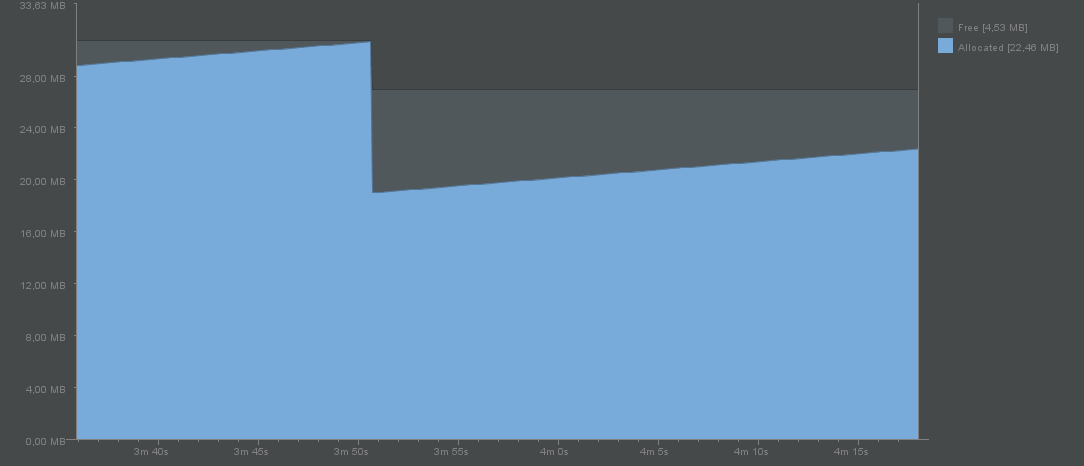
\includegraphics[width=1\linewidth]{figures/ch10/22.png}\label{fig10.22}}
	\\
	\subfloat[Memory usage during a record plotting. We force two GC calls as they can be seen considering the the first big step and the second small one.]{	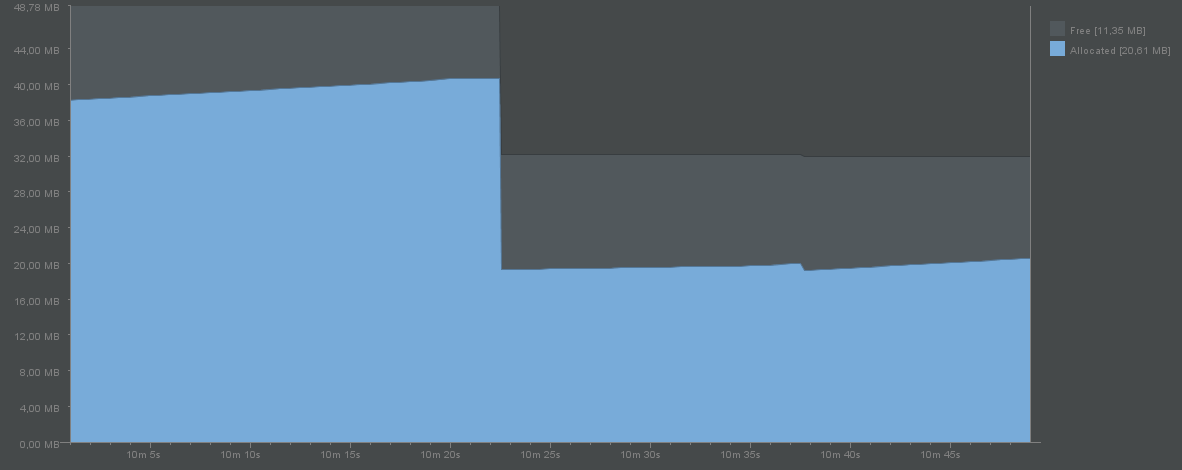
\includegraphics[width=1\linewidth]{figures/ch10/23.png}\label{fig10.23}}
	\caption{Two memory usage views during a normal app execution, on the second figure a GC is called before the memory reach the heap}  
	\label{fig22.15ab}
\end{figure}
In the figure \ref{fig10.23} we can see a system GC call triggered when the application reaches the upper bound of the memory heap allocated for the application process. The OS waits to trigger a GC call until the process fills and hit the memory heap. Lollipop GC policy is then completely different from the Jelly Bean (Samsung N7000). It allows application to fill the heap and only after that it triggers a GC and estimates the new heap size. For a test purpose We choose to trigger a GC call before the process can fill the heap. You can see in figure \ref{fig10.23} that the forced GC call cleared the heap (the first big step) and resized the heap according to the resource need. After that the heap keeps being filled with new allocations and also old allocations, but at 10m37s we triggered another forced GC call (second small step). We can now realize for real how many resources are really used during plotting phase and how many are just put in the GC queue. If we keep calling forced GC, probably we would achieve the same behaviour as the one observed on the Samsung N7000 (a series of memory waves).
\newpage
A detailed view of memory allocation by RAM types is shown below:
\begin{figure}[h!]
	\centering	
	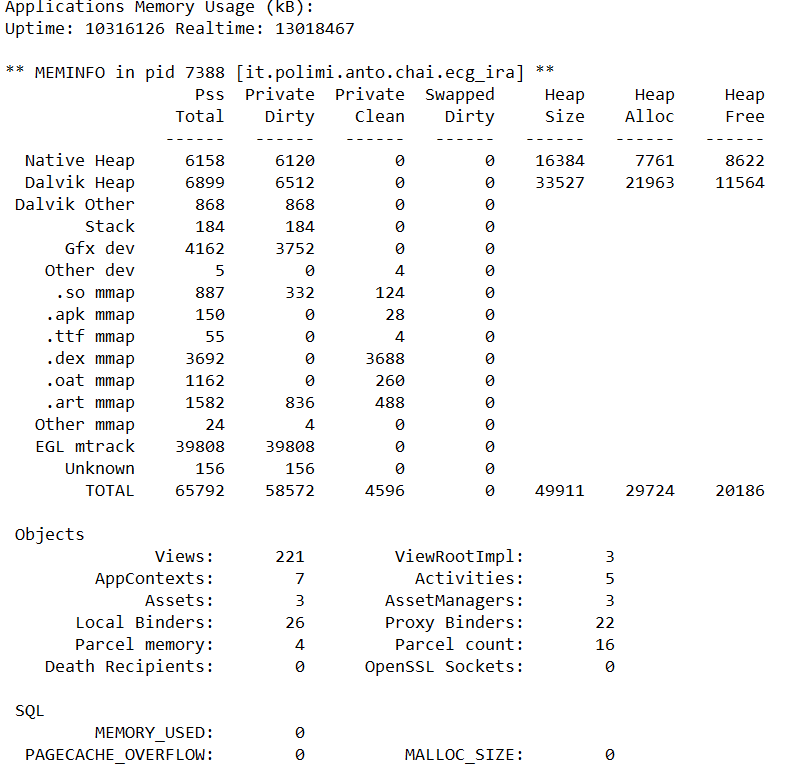
\includegraphics[width=0.6\linewidth]{figures/ch10/24.png}
	\caption{ Memory usage details by RAM types.}  
	\label{fig10.24}
\end{figure}
As the plotting state requires more drawings and dynamic data usage (updates of data structure and views updates) there is an obvious increase of resources needs.
\subparagraph{Analysis state}
Considering how the GC behaves the analysis state is kind of predictable.
\begin{figure}[!htb]
	\centering
	\subfloat[Memory usage when a record analysis is called. The step in the memory usage graph is due to the buffer allocation for the record.]{	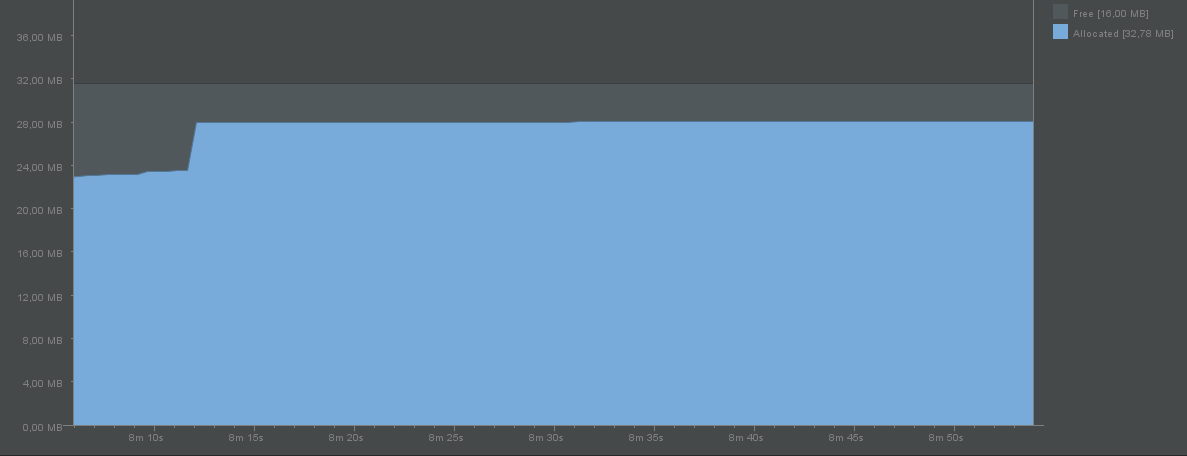
\includegraphics[width=1\linewidth]{figures/ch10/25.png}\label{fig10.25}}
	\\
	\subfloat[Memory usage when a record analysis is called. The step in the memory usage graph is due to the analysis algorithm running on the record.]{	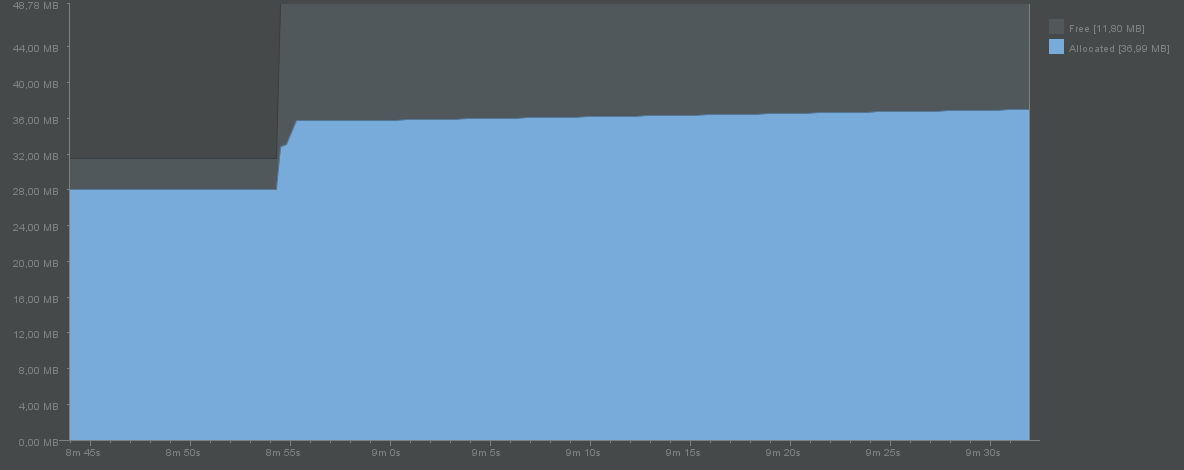
\includegraphics[width=1\linewidth]{figures/ch10/26.png}\label{fig10.26}}
	\caption{Two memory usage views during the execution of the analysis algorithms, on the first figure \ref{fig10.25} the step sign the execution satrting point, in figure \ref{fig10.26} the step is due to the end of the execution}  
	\label{fig25.15ab}
\end{figure}
Instead of calling a GC after the buffer becomes useless as the analysis algorithm finishes, the OS instantiates more memory heap for the process as it needs and sets up a new and higher upper bound. The GC call will be triggered only when the new bound is reached. We already know that most of the allocated resources are to be garbage collected but since the limit of the heap size will not be hit no GC calls will be triggered. We can observe that all the resources used during  the analysis are kept in memory.
\begin{figure}[ht]
	\centering	
	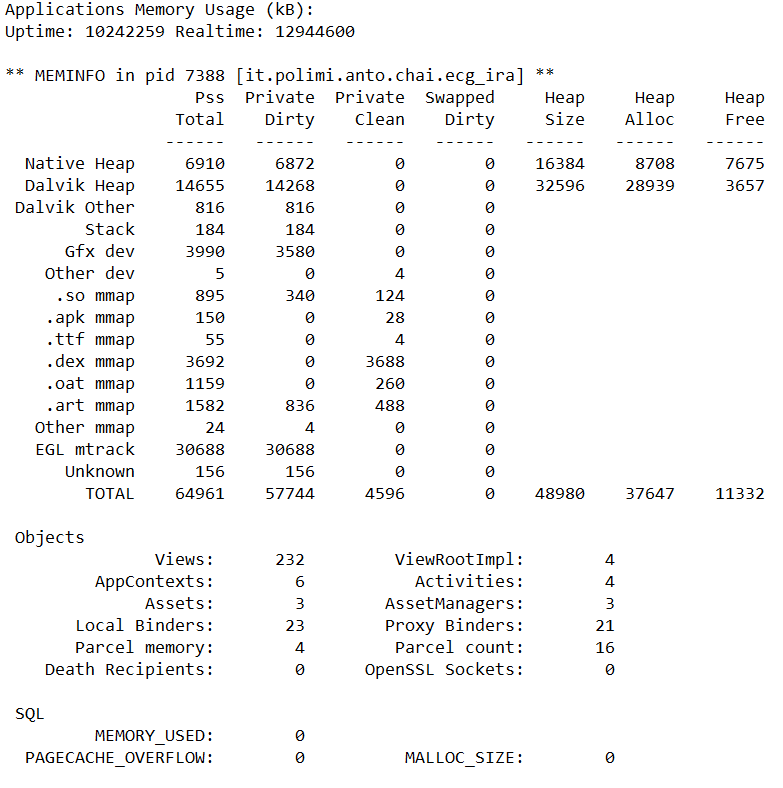
\includegraphics[width=0.6\linewidth]{figures/ch10/27.png}
	\caption{Memory usage when a record analysis is called. The memory usage is divide by RAM types.}  
	\label{fig10.27}
\end{figure}
\newpage
Due to the creation of the copy record buffer the Dalvik Private Dirty is doubled (from 6512 kB in plotting state to 14268 kB in analysis state) and since we pause all the views the EGL mTrack is reduced (less views need memory).
\newline
The overall memory usage keeps being the same also for the OnePlus X device, even if on this device the GC behaviour is completely different, the resource used are limited and deallocated when there is no more need of them. Having  less GC calls improved the application performance since any GC call affects and keeps the CPU busy for while. Also the use of an additional graphical layer improves the application responsiveness and performance, but it also comes with a more intensive memory usage that not all devices can afford. In case of the OnePlus X hardware memory limitation is not a great deal with its 3GB RAM memory, nor the performance limitation is really a limit, but since the application has to be run on other devices as well, these principles should always be considered.
\subsubsection{CPU}
The CPU performance tests were done by executing the same actions on the same views. We decide to provide CPU usage during an application run on different devices. As in the memory tests we decide to track CPU usage with the application on the three different states:\\
Idle state, Plotting state and Analysis state. The CPU usage is reported into percentages and is related to the amount of CPU power used by the Kernel and by the User (in this case the User is the application process).
\paragraph{Samsung Galaxy N7000}
This device has a Dual-core 1.4 GHz Cortex-A9, performed fairly well even with its large screen 5.3 inches and its 800x1280 pixels (285 ppi pixel density).
\subparagraph{Idle state}
During Idle state, when the application is simply kept on foreground on a static screen, we can observe there are no cpu usage leakage.
\begin{figure}[ht!]
	\centering	
	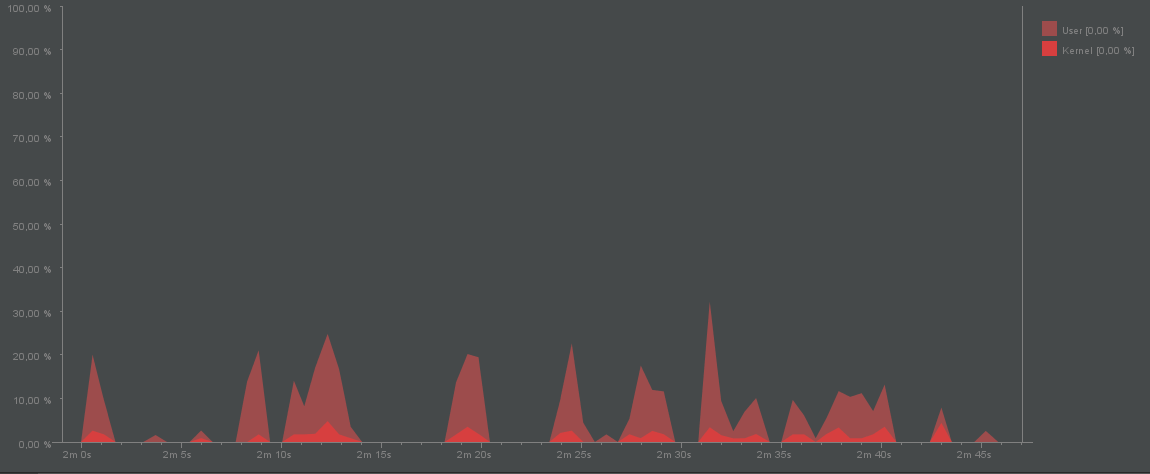
\includegraphics[width=1\linewidth]{figures/ch10/28.png}
	\caption{Cpu usage during idle state, the application is on foreground on a static page.}  
	\label{fig10.28}
\end{figure}
The peaks in the figure 10.28 are due to the user’s interaction with the listview, otherwise in case of no interaction at all the graph is plain. At each peak the ListAdapter (in this case the RecycleViewAdapter) instantiates and so inflates the next item list represented by a record in the list so that the user can visualize it on the scrolling action.
\subparagraph{Plotting state}
During plotting state the CPU usage results to be quite constant. In the figure \ref{fig10.29}, we can observe that it never exceed 60\%.
\begin{figure}[ht!]
	\centering	
	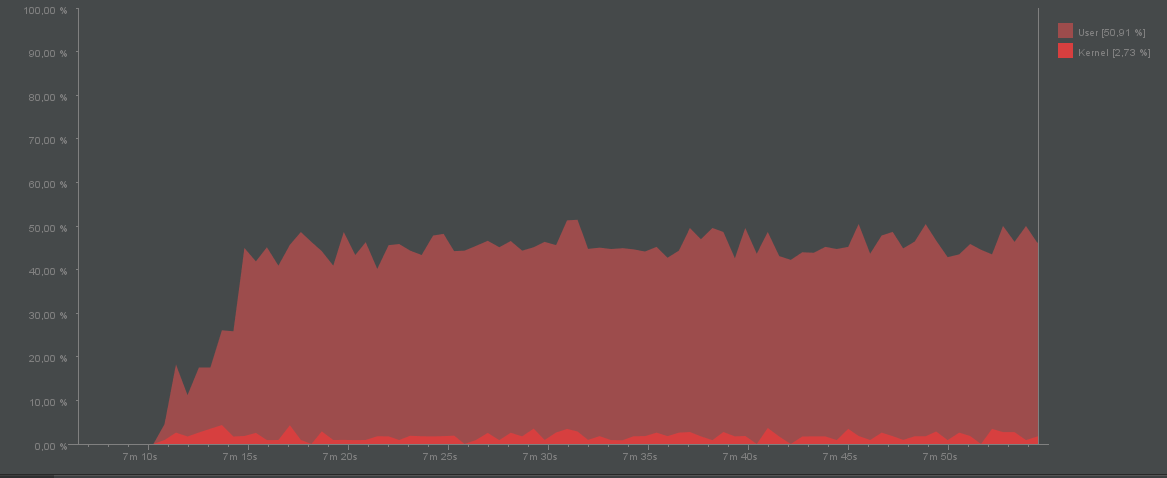
\includegraphics[width=1\linewidth]{figures/ch10/29.png}
	\caption{Cpu usage when a record is plot on screen.}  
	\label{fig10.29}
\end{figure}
At minute 7m10s we selected the record 100.dat and opened it. The plotting screen keeps the cpu quite busy at a constant rate (between 40\% and 58\%) . This value doesn’t change and it is independent from the user’s interaction (not like the listView which requires cpu at each user’s interaction as scrolling). Also during the automatic scrolling of the ECG strip, the cpu usage keeps being the same. This can be explained by observing that this screen and all the views were completely customized and implemented by us. As the views on screen are plotting canvases and to get the animation features we are forced to use a second thread to manage the drawings. By this way the screen content is redrawn as often as it is possible according to the maximum frame rate set by the user but compatible the frame rate the thread can get.\\
As soon as the user closes the Plotting screen, the cpu usage dropped and resources are kept free.
\begin{figure}[h!]
	\centering	
	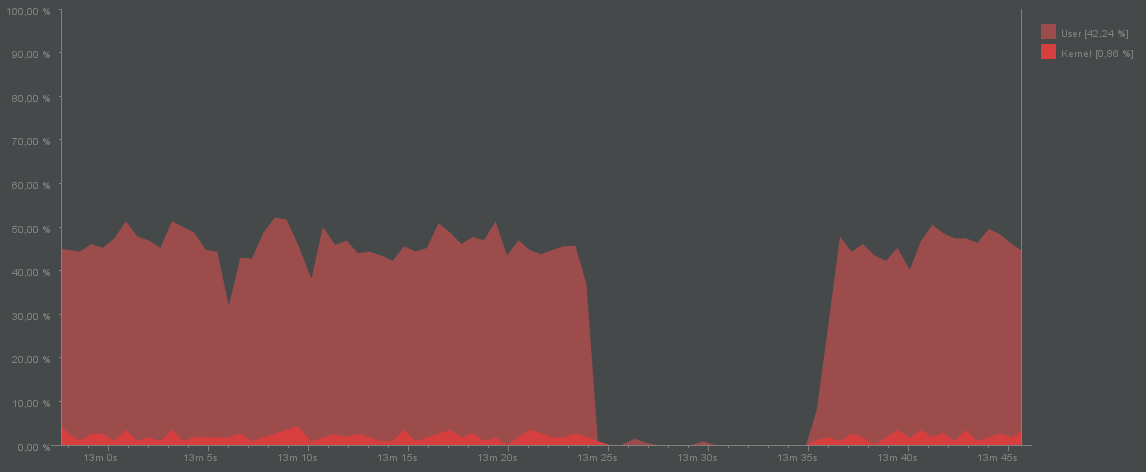
\includegraphics[width=1\linewidth]{figures/ch10/30.png}
	\caption{Cpu usage when we close a plotting screen and reopen it.}  
	\label{fig10.30}
\end{figure}
In figure 10.30 at minute 13m25s we closed the Activity with the ECG strip plot.  We can observe that the application released immediately the cpu resources as they are no more needed. Also all the drawing threads are killed and streams closed. But as at minute 13m35s we reopened another record, the resources are reallocated and the new views show ups. New drawing threads are instantiated and a new data stream is opened to read the new record data.
\subparagraph{Analysis state}
Interesting results comes from the Analysis state. As you can see in the figure 10.31, at minute 8m30s we launched an analysis command. The down peak is due to the drawing thread freezing as we stop all drawing for a while. If during the memory test we observed an increasing of memory allocation, here there is no significant changes into the cpu usage. We just pause the drawing thread and launch an AsyncTask to compute the analysis over the ECG record.
\begin{figure}[h!]
	\centering	
	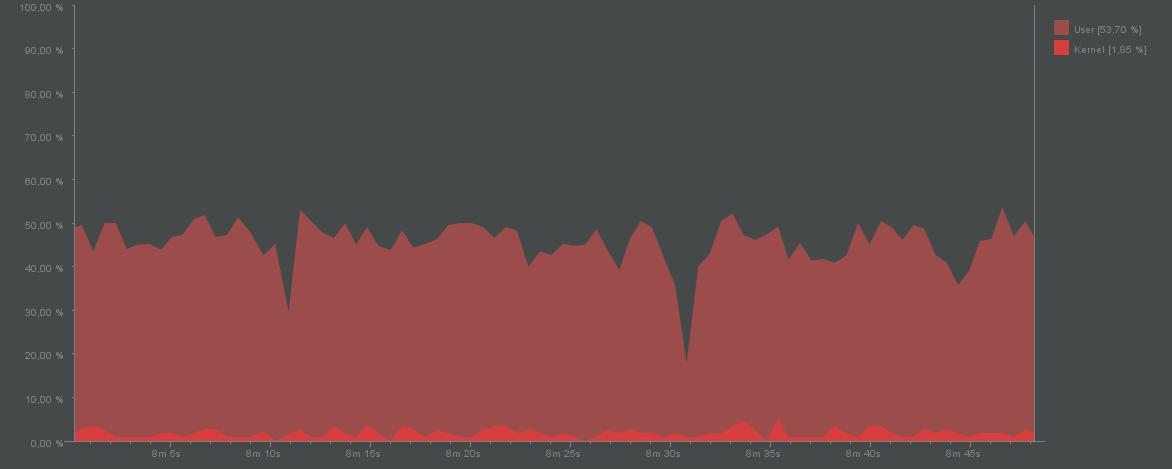
\includegraphics[width=1\linewidth]{figures/ch10/31.png}
	\caption{CPU usage during analysis state. An analysis command is launched over an ECG record strip.}  
	\label{fig10.31}
\end{figure}
\paragraph{OnePlus X}
CPU usage on this device didn’t differ that much on the previous results on the Samsung N7000. The application achieved same performance and never exceeded 60\% of the CPU capabilities. The graph suggests that in the Quad-core the average CPU usage is also smaller than the one found on the Samsung N7000’s Dual-core.
\subparagraph{Idle state}
On idle state the cpu usage is reduced at minimum. Less than 2\% of CPU power usage is registered on static screen pages.
\begin{figure}[h!]
	\centering	
	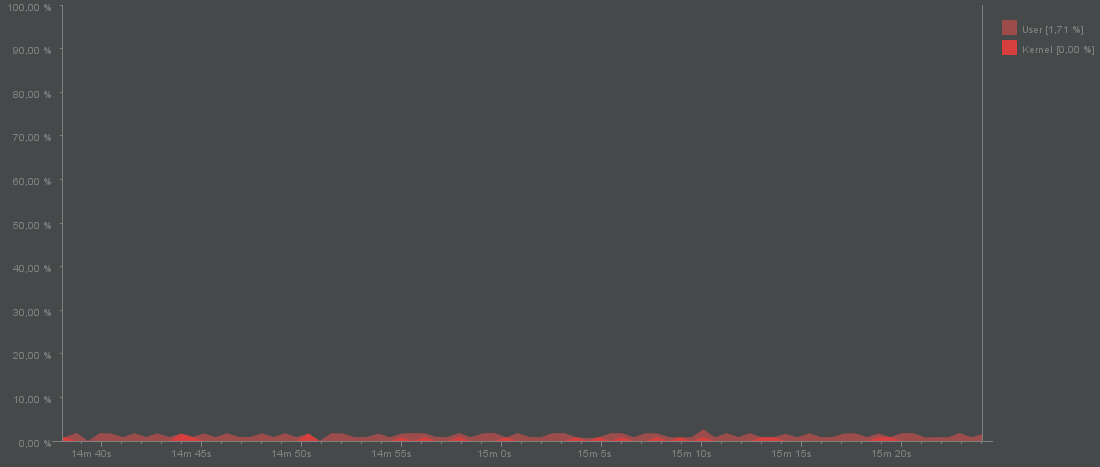
\includegraphics[width=1\linewidth]{figures/ch10/32.png}
	\caption{CPU usage on idle pages(app open on static screen page)}  
	\label{fig10.32}
\end{figure}
\subparagraph{Plotting state}
During the plotting of a record the application CPU usage is constant in  a range between 25\% to 45\%.
\begin{figure}[h!]
	\centering	
	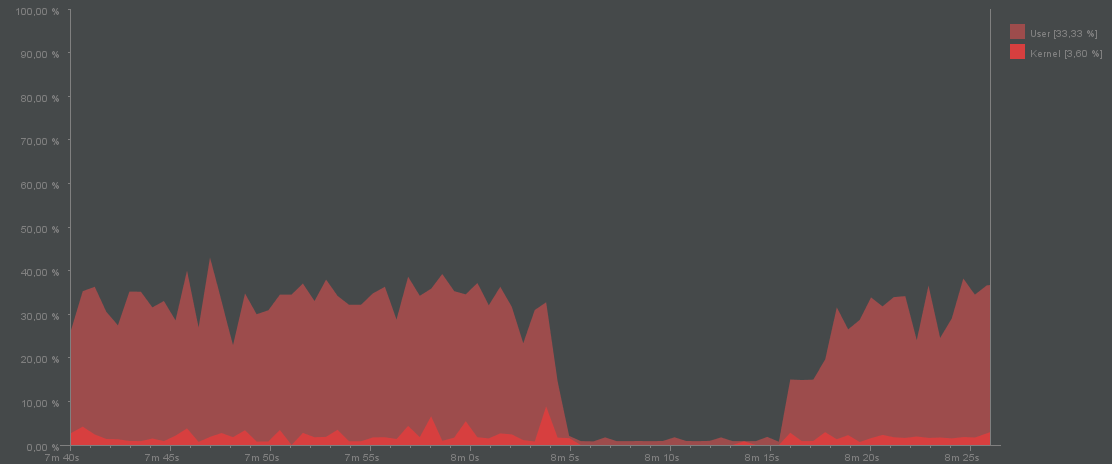
\includegraphics[width=1\linewidth]{figures/ch10/33.png}
	\caption{CPU usage during a record plotting)}  
	\label{fig10.33}
\end{figure}
The slope down is due to a change in activity view. The Record Activity is closed at minute 8m5s. The process (and all the threads)  in charge to draw the ECG signals is killed so also resources are released as well. At minute 8m15s another record is opened and new resources and threads  are allocated.\\
We can observe that the overall cpu usage on the OnePlus X device is on average less than the average cpu usage on the Samsung N7000, even if the application overall performance results to have the same behaviour.
\subparagraph{Analysis state}
During the analysis state the maximum cpu usage is not changed. It worth mentioning that even if there is no significant change in the \% of cpu usage, on the OnePlus X the execution time of analysis is much shorter.
\begin{figure}[h!]
	\centering	
	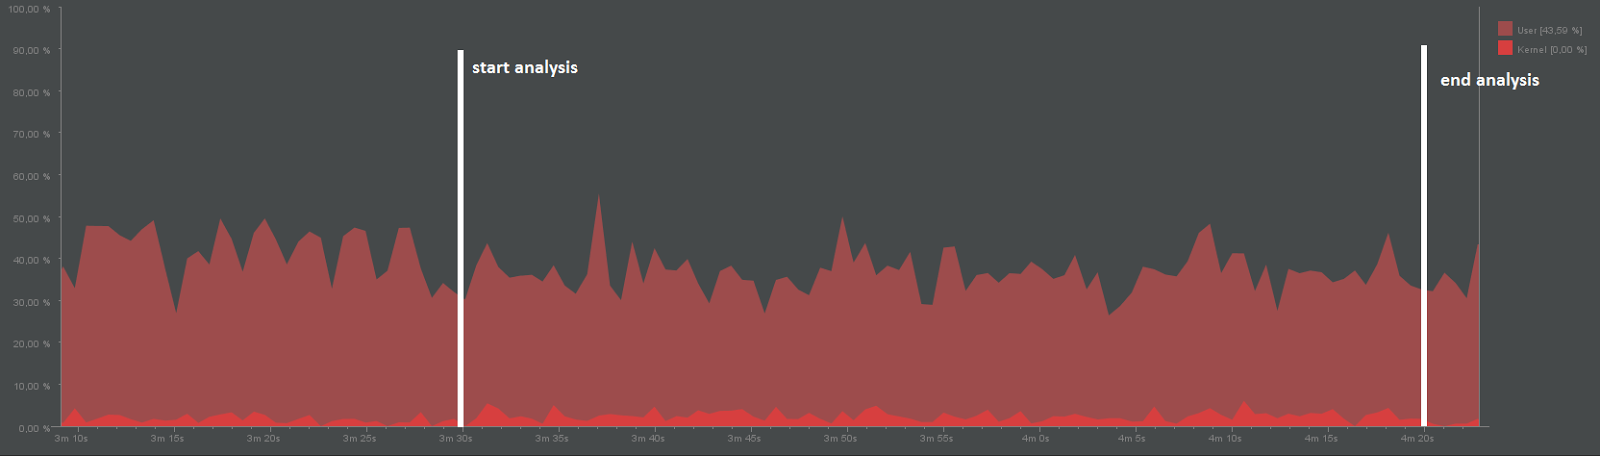
\includegraphics[width=1\linewidth]{figures/ch10/34.png}
	\caption{usage when the  analysis algorithm is launched over a record)}  
	\label{fig10.34}
\end{figure}
In the figure \ref{fig10.34} during a plotting state the analysis is launched at minute 3m30s (first white bar). The process terminates at minute 4m20s as shown by the second white bar.
\subsection{Response Time}
We performed a test about the response  time and the time spent by the processor to load the plotting page and the time spent on executing the analysis algorithm.\\
To have accurate measurements we put inside the application additional lines of code as checkpoints.\\
Android OS offers an utility class to measure execution time of methods that is the TimingLogger class.\\
As documented into the Android references guide the class is used as follows:
\begin{lstlisting}
     TimingLogger timings = new TimingLogger(TAG,"methodA");
          //do some work A
          timings.addSplit("work A");
          // do some work 
          timings.addSplit("work B");
          //do some work C
          timings.addSplit("work C");
          timings.dumpToLog();
\end{lstlisting}
After a class declaration we split the time between the methods we want to check the execution time.\
We used such a class to measure the longest operations within ECG-ira, that is when we load the record into memory and when we execute the analysis on the record.
\begin{lstlisting}
//A timingLogger implementation to measure the execution time of the two //longest processes.
@Override
protected Boolean doInBackground(Void params) {
TimingLogger timeLogger = new TimingLogger("it.polimi.anto.chai.ecg_ira.Activity.AsyncTask", "RECORD ANALYSIS");
short[] result = parser.getSamplesForAnalysis(index);
timeLogger.addSplit("sample extraction from file to memory");
Analysis.execute(result, rate);
timeLogger.addSplit("analysis execution");
timeLogger.dumoToLog();
}
\end{lstlisting}
The same code was executed on different devices and as expected the OnePlus X performed much better in term of execution time.\\
Below is reported the execution time in milliseconds for the sample extraction from the .dat file to the memory and the time spent to execute the analysis on the record.\\
\begin{table}[h]
\begin{tabularx}{\textwidth}{|X|X|X|}
	\hline
	\textbf{\#of executions} & \textbf{Memory load (ms)} &\textbf{Analysis execution (ms)}  \\ \hline
	run1 & 115 & 55038  \\ \hline
	run2 & 101 & 46429 \\ \hline
	run3 & 98 & 47775 \\ \hline
	run4 & 87 & 47910 \\ \hline
	run5 & 92 & 47087 \\ \hline
	average & 98.6 & 48847.8 \\ \hline
	
\end{tabularx}
\caption{Execution time for a record load in memory and its analysis on the OnePlus X device}
\label{tab10.2}
\end{table}
The memory load on the OnePlus X is extremely fast taking on average  about 0.1 second (98.6 milliseconds) on a record which lasts 30 minutes and dimension 1.9 MB. \\
The analysis method is the longest in term of execution time. On average on the OnePlus X it takes about 48 seconds to execute (48.847 milliseconds). The results are not precise as the execution time takes in consideration many other independent external factors. The overall time can be less than the average or even much higher due to the number of processes running on background. Five runs are  not exhaustive at all for a detailed performance analysis  but it gives a general view of the performance we can get during a normal usage of the phone.
\begin{table}
\begin{tabularx}{\textwidth}{|X|X|X|}
	 \hline
	\textbf{\#of executions} & \textbf{Memory load (ms)} &\textbf{Analysis execution (ms)}  \\ \hline
	run1 & 275 & 121483  \\ \hline
	run2 & 320 & 128352 \\ \hline
	run3 & 358 & 136027 \\ \hline
	run4 & 242 & 144923 \\ \hline
	run5 & 334 & 156327 \\ \hline
	average & 305.8 & 137422.4 \\ \hline

\end{tabularx}
	\caption{Execution time for a record load in memory and its analysis on the Samsung N7000 device}
	\label{tab10.3}
\end{table}
The execution time on the Samsung N7000 are three time slower on average  with a memory load time of 0.3 seconds and an Analysis execution time of 2.30 minutes.\\
We observed that during other tests the application overall behaviour with respect to memory usage and amount of CPU usage is regular and the application doesn’t show any kind of leakages nor crashes. The huge difference in the execution time is mostly due to the difference in the hardware and software strategy. The OnePlus X quad-core is obviously performing much faster than the Dual-core of the Samsung N7000. Also the availability of 3 GB of RAM can allow the OS  not to call the GC as often as the OS on the Samsung device which has limited 1GB RAM to be shared across all the applications.